\documentclass[hyperref={bookmarks=false},aspectratio=169]{beamer}
\usepackage{hyperref,ragged2e,amsmath,amssymb,url,bm}
\usepackage{graphicx,booktabs,array}
\usepackage{tikz}
\usetikzlibrary{arrows.meta,positioning,calc,shapes.geometric,decorations.pathreplacing,matrix}
\graphicspath{{crops/}}
\usetheme{Goettingen}
% --- Paleta: azul profundo, dorado y papiro crema ---
\definecolor{azul}{HTML}{15437C}
\definecolor{azuloscuro}{HTML}{0B1F3A}
\definecolor{celeste}{HTML}{5694D6}
\definecolor{dorado}{RGB}{196,154,60}
\definecolor{papiro}{RGB}{246,239,220}
\definecolor{gris}{RGB}{70,78,96}
\setbeamercolor{structure}{fg=azul}
\setbeamertemplate{sidebar canvas right}[vertical shading][top=azul,bottom=azuloscuro]
\setbeamercolor{title in sidebar}{fg=dorado}
\setbeamercolor{author in sidebar}{fg=papiro}
\setbeamercolor{section in sidebar}{fg=papiro}
\setbeamercolor{section in sidebar shaded}{fg=dorado!70!papiro}
\setbeamercolor{subsection in sidebar}{fg=papiro}
\setbeamercolor{subsection in sidebar shaded}{fg=dorado!70!papiro}
\let\raggedright\justifying
\setlength{\RaggedRightRightskip}{0pt plus 1fil}
\setbeamertemplate{background canvas}{
\includegraphics[width=\paperwidth,height=\paperheight]{papiro.jpg}}
\setbeamercolor{normal text}{fg=black!88!azuloscuro}
\setbeamercolor{frametitle}{fg=azul}
\setbeamerfont{frametitle}{series=\bfseries}
\setbeamertemplate{section in toc shaded}{\leavevmode{\color{gris}\inserttocsection}\par}
\setbeamercolor{title}{fg=azul}
\setbeamercolor{subtitle}{fg=gris}
\setbeamercolor{item projected}{bg=azul,fg=papiro}
\setbeamertemplate{itemize item}{\small\textcolor{dorado}{$\blacktriangleright$}}
\setbeamertemplate{navigation symbols}{}
% --- Español + hebreo + griego (XeLaTeX) ---
\usepackage[bidi=default]{babel}
\babelprovide[import,main]{spanish}
\babelprovide[import]{hebrew}
\babelprovide[import]{ancientgreek}
\babelfont[hebrew]{sf}[Path=fonts/, BoldFont=NotoHebrewSans-700.ttf]{NotoHebrewSans-400.ttf}
\babelfont[hebrew]{rm}[Path=fonts/, BoldFont=NotoHebrewSans-700.ttf]{NotoHebrewSans-400.ttf}
\babelfont[ancientgreek]{sf}[Path=fonts/]{GFSPorson.otf}
\babelfont[ancientgreek]{rm}[Path=fonts/]{GFSPorson.otf}
\newcommand{\heb}[1]{\mbox{\foreignlanguage{hebrew}{#1}}}
\newcommand{\grc}[1]{\foreignlanguage{ancientgreek}{#1}}
\newcommand{\SENOR}{S{\fontsize{0.78em}{1em}\selectfont EÑOR}}
% --- Citas (cuadro de un solo color), imágenes, referencias ---
\usepackage[most]{tcolorbox}
\newtcolorbox{cita}[1][]{enhanced, colback=azul!7!papiro, opacityback=0.85, colframe=azul,
  boxrule=0pt, leftrule=2.5pt, arc=0pt, left=6pt, right=6pt, top=4pt, bottom=4pt,
  before skip=4pt, after skip=6pt, fontupper=\small\itshape, #1}
\newcommand{\fuente}[1]{\par\hfill{\upshape\bfseries\footnotesize\textcolor{azul}{#1}}}
\makeatletter
\newcommand{\fotolado}[2]{%
  \begin{tikzpicture}[remember picture,overlay]
    \node[anchor=north east,inner sep=0pt] (foto) at ([xshift=-\beamer@sidebarwidth]current page.north east)
      {\includegraphics[height=\paperheight]{#1}};
    \node[anchor=south east,inner sep=2pt,text=papiro,fill=azuloscuro,fill opacity=0.6,text opacity=1,
      font=\fontsize{4.5}{5.5}\selectfont,align=right,text width=4.2cm] at ([xshift=-3pt,yshift=3pt]foto.south east)
      {\textit{Nota.} #2};
  \end{tikzpicture}}
\makeatother
\newcommand{\refapa}[1]{\par{\RaggedRight\hangindent=1.2em\hangafter=1\noindent #1\par}\vspace{3pt}}
\usepackage{xurl}\urlstyle{same}
\newcommand{\destacar}[1]{\textbf{\textcolor{azul}{#1}}}
\newcommand{\precision}[1]{{\footnotesize\color{gris}\textbf{Precisión:} #1}}
\tikzset{caja/.style={draw=azul,line width=0.8pt,fill=papiro,fill opacity=0.92,text opacity=1,rounded corners=3pt,inner sep=5pt,font=\scriptsize}}
\title[La misericordia]{\bfseries{La misericordia de Dios}}
\subtitle{``¡\SENOR! ¡\SENOR! fuerte, misericordioso y piadoso'' (Éx 34:6)}
\author{}\institute{}\date{}
\titlegraphic{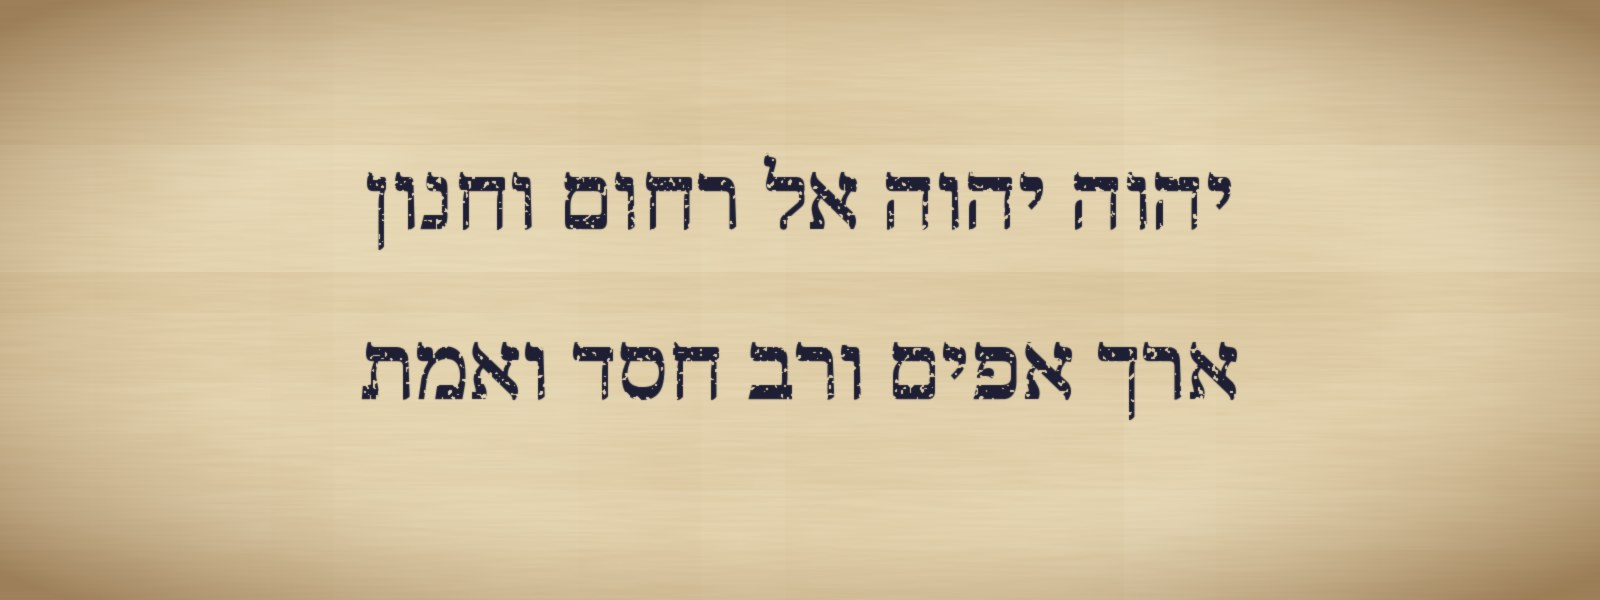
\includegraphics[width=0.80\linewidth,height=0.36\textheight,keepaspectratio]{portada.jpg}\\[-1pt]
  {\fontsize{5}{6}\selectfont\color{gris}\textit{Nota.} Elaboración propia: Éx 34:6 en texto hebreo consonántico (BHS).}}
\AtBeginSection[]{\begin{frame}\frametitle{Contenidos}\tableofcontents[currentsection]\end{frame}}
\begin{document}
\frame{\titlepage}

\begin{frame}\frametitle{Contenidos}\tableofcontents\end{frame}

% ------------------------------------------------------------------
\section{Contexto}

\begin{frame}{¿Qué significa ``tiempo''?}
\begin{columns}[c,onlytextwidth]
\begin{column}{0.50\textwidth}
\centering
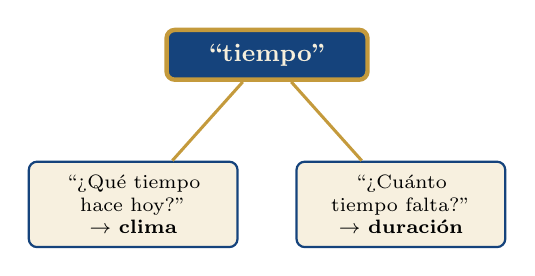
\begin{tikzpicture}[font=\scriptsize]
 \node[draw=dorado,line width=1.6pt,fill=azul,text=papiro,rounded corners=3pt,text width=2.2cm,align=center,inner sep=5pt,font=\small\bfseries] (t) at (0,0) {``tiempo''};
 \node[caja,text width=2.3cm,align=center] (a) at (-1.7,-1.9) {``¿Qué tiempo hace hoy?''\\ $\rightarrow$ \textbf{clima}};
 \node[caja,text width=2.3cm,align=center] (b) at (1.7,-1.9) {``¿Cuánto tiempo falta?''\\ $\rightarrow$ \textbf{duración}};
 \draw[dorado,line width=1.1pt] (t)--(a); \draw[dorado,line width=1.1pt] (t)--(b);
\end{tikzpicture}
\end{column}
\begin{column}{0.48\textwidth}\small
\begin{itemize}
\item En español, una sola palabra junta conceptos distintos; el contexto decide cuál.
\item Con la Escritura pasa lo inverso: \destacar{varias palabras} hebreas y griegas terminaron traducidas con \destacar{una sola} palabra española.
\item Así ocurre con ``misericordia''.
\end{itemize}
\end{column}
\end{columns}
\end{frame}

\begin{frame}{``Misericordia'' en la Biblia}
\begin{columns}[c,onlytextwidth]
\begin{column}{0.42\textwidth}\footnotesize
\begin{itemize}
\item Tu material: \destacar{más de 290 veces}, traduciendo \destacar{6 palabras} del original.
\item RVR1960: ``misericordia(s)'' \textbf{403 veces} (331 AT, 72 NT); con ``misericordioso(a)'', \textbf{432 veces} en 403 versículos.
\item Detrás hay \destacar{8 raíces hebreas, 2 términos arameos y 4 familias griegas}.
\end{itemize}
\end{column}
\begin{column}{0.56\textwidth}
\scriptsize\renewcommand{\arraystretch}{1.12}
\begin{tabular}{@{}>{\RaggedRight\arraybackslash}p{3.3cm}>{\RaggedRight\arraybackslash}p{2.2cm}r@{}}
\toprule
\textbf{Raíz o familia} & \textbf{Sentido base} & \textbf{Vv.} \\ \midrule
\heb{חסד} \emph{jésed}, \emph{jasid} & amor leal & $\approx$\,220 \\
\heb{רחם} \emph{rajamím}, \emph{rajam}, \emph{rajum} & entrañas & $\approx$\,77 \\
\heb{חנן} \emph{janán}, \emph{jannun}, \emph{tejinná} & gracia, súplica & $\approx$\,63 \\
\heb{חוס} \emph{jus} & tener lástima & $\approx$\,11 \\
\heb{חמל} \emph{jamal}, \emph{jemlá} & perdonar la vida & 10 \\
\heb{נחם} \emph{najam}; \heb{טוב עין} \emph{tov ayin} & conmoverse; ``buen ojo'' & 1; 1 \\
arameo \emph{rajamín}, \emph{mijan} & compasión; gracia & 1; 1 \\
\grc{ἔλεος}, \grc{ἐλεέω} y derivados & compasión activa & 58 \\
\grc{σπλάγχνα} y derivados & entrañas & 11 \\
\grc{οἰκτιρμός}, \grc{οἰκτίρμων} & compasión & 6 \\
\grc{ὅσιος} (Hch 13:34) & lealtad (= \emph{jésed}) & 1 \\
\bottomrule
\end{tabular}\par\smallskip
{\tiny\color{gris}Versículos de la RVR1960 con ``misericord-'' donde aparece la raíz; un versículo puede tener dos.}
\end{column}
\end{columns}
\precision{conteo propio (RVR1960, BHS y NA27 con Strong), sin los títulos de sección; verificar en e-Sword.}
\end{frame}

\begin{frame}{Babel: la ``puerta de dios''}
\begin{columns}[c,onlytextwidth]
\begin{column}{0.50\textwidth}
\begin{cita}Por esto fue llamado el nombre de ella Babel, porque allí confundió \SENOR{} el lenguaje de toda la tierra, y desde allí los esparció sobre la faz de toda la tierra.\fuente{(Gn 11:9, RVR1960)}\end{cita}
\begin{center}\heb{עַל־כֵּן קָרָא שְׁמָהּ בָּבֶל כִּי־שָׁם בָּלַל יְהוָה}\end{center}
\end{column}
\begin{column}{0.48\textwidth}
\scriptsize\renewcommand{\arraystretch}{1.2}
\begin{tabular}{@{}>{\RaggedRight\arraybackslash}p{1.9cm}>{\RaggedRight\arraybackslash}p{3.6cm}@{}}
\toprule
\textbf{Acadio} & \emph{Bāb-ilim}: \emph{bāb} ``puerta'', \emph{ilim} ``de dios''. Para Babilonia, su ciudad unía el cielo y la tierra. \\
\textbf{Hebreo} & \heb{בָּלַל} \emph{balal}: ``confundir, mezclar''. Moisés hace un juego de palabras: la ``puerta de dios'' es ``confusión''. \\
\bottomrule
\end{tabular}\par\medskip
\small ``Hagámonos un nombre'' (Gn 11:4): el hombre busca su gloria y fabrica su propio acceso al cielo.\par\smallskip
\precision{la etimología acadia y el juego de palabras siguen a Wenham (1987) y HALOT.}
\end{column}
\end{columns}
\end{frame}

\begin{frame}{La gloria cambiada}
\begin{columns}[t,onlytextwidth]
\begin{column}{0.49\textwidth}
\begin{cita}Profesando ser sabios, se hicieron necios, y cambiaron la gloria del Dios incorruptible en semejanza de imagen de hombre corruptible, de aves, de cuadrúpedos y de reptiles.\fuente{(Ro 1:22--23, RVR1960)}\end{cita}
\scriptsize\grc{ἤλλαξαν τὴν δόξαν τοῦ ἀφθάρτου θεοῦ}: ``cambiaron la gloria del Dios incorruptible''. \grc{ἀλλάσσω}, ``cambiar, trocar''.
\end{column}
\begin{column}{0.49\textwidth}
\begin{cita}Hicieron becerro en Horeb, Se postraron ante una imagen de fundición. Así cambiaron su gloria Por la imagen de un buey que come hierba.\fuente{(Sal 106:19--20, RVR1960)}\end{cita}
\scriptsize\heb{וַיָּמִירוּ אֶת־כְּבוֹדָם בְּתַבְנִית שׁוֹר} (\emph{vayyamiru et-kevodam}): ``cambiaron su gloria'' (\heb{מור}, ``trocar''). Pablo usa el lenguaje del Salmo: lo que hizo Israel en el Sinaí es lo que hace toda la humanidad.
\end{column}
\end{columns}
\precision{el eco de Sal 106:20 (LXX 105:20, \grc{ἠλλάξαντο τὴν δόξαν αὐτῶν}) en Ro 1:23 lo reconocen los comentaristas (Moo, 1996).}
\end{frame}

\begin{frame}{De la gloria del Eterno a la gloria del Eterno}
\centering
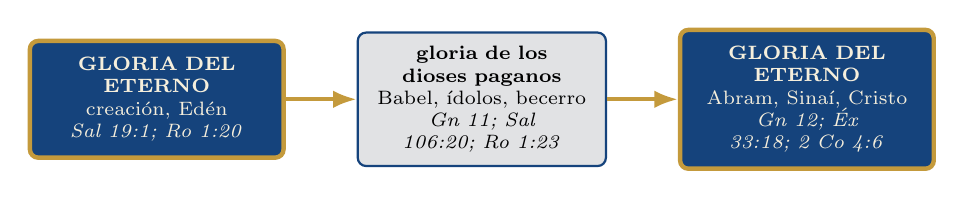
\begin{tikzpicture}[font=\scriptsize,node distance=0.9cm]
 \node[draw=dorado,line width=1.6pt,fill=azul,text=papiro,rounded corners=3pt,text width=2.8cm,align=center,inner sep=6pt] (a) {\textbf{GLORIA DEL ETERNO}\\ creación, Edén\\ \emph{Sal 19:1; Ro 1:20}};
 \node[caja,text width=2.8cm,align=center,fill=gris!18,right=of a] (b) {\textbf{gloria de los dioses paganos}\\ Babel, ídolos, becerro\\ \emph{Gn 11; Sal 106:20; Ro 1:23}};
 \node[draw=dorado,line width=1.6pt,fill=azul,text=papiro,rounded corners=3pt,text width=2.8cm,align=center,inner sep=6pt,right=of b] (c) {\textbf{GLORIA DEL ETERNO}\\ Abram, Sinaí, Cristo\\ \emph{Gn 12; Éx 33:18; 2 Co 4:6}};
 \draw[-{Latex[length=3mm]},dorado,line width=1.4pt] (a)--(b);
 \draw[-{Latex[length=3mm]},dorado,line width=1.4pt] (b)--(c);
\end{tikzpicture}\par\medskip
\begin{tcolorbox}[colback=papiro,colframe=dorado,boxrule=1.2pt,arc=3pt]
\centering\small ``Desde Abram hacia adelante se comienza a llamar a los hombres a \destacar{elegir la gloria del Dios verdadero}.''
\end{tcolorbox}
\small\RaggedRight Se dan los primeros pasos para formar un pueblo libre de pensamientos errados: un pueblo que tomaría conceptos de los pueblos antiguos, corrigiendo su error y su significado.
\end{frame}

\begin{frame}{El encuentro de Abram y el Eterno}
\begin{columns}[t,onlytextwidth]
\begin{column}{0.52\textwidth}
\begin{cita}Pero \SENOR{} había dicho a Abram: Vete de tu tierra y de tu parentela, y de la casa de tu padre, a la tierra que te mostraré. Y haré de ti una nación grande, y te bendeciré, y engrandeceré tu nombre, y serás bendición.\fuente{(Gn 12:1--2, RVR1960)}\end{cita}
\scriptsize\heb{וַאֲגַדְּלָה שְׁמֶךָ} (\emph{va'agaddelá shemeja}): ``y engrandeceré tu nombre''. En Babel el hombre quería ``hacerse un nombre'' (Gn 11:4, \heb{שֵׁם}); a Abram, Dios se lo da.
\end{column}
\begin{column}{0.46\textwidth}
\begin{cita}Y pasó Abram por aquella tierra hasta el lugar de Siquem, hasta el encino de More; y el cananeo estaba entonces en la tierra. Y apareció \SENOR{} a Abram\ldots{} Y edificó allí un altar a \SENOR.\fuente{(Gn 12:6--7, RVR1960)}\end{cita}
\small En medio del culto cananeo, Abram levanta un altar al \SENOR: su primer ``no'' a los dioses de la tierra.
\end{column}
\end{columns}
\precision{la lectura ``Babel busca un nombre / Abram lo recibe'' es común entre los comentaristas (Wenham, 1987); el contraste con el culto cananeo de Siquem es lectura propia de esta serie.}
\end{frame}

% ------------------------------------------------------------------
\section{Éxodo 34}

\begin{frame}{Después del becerro}
\centering
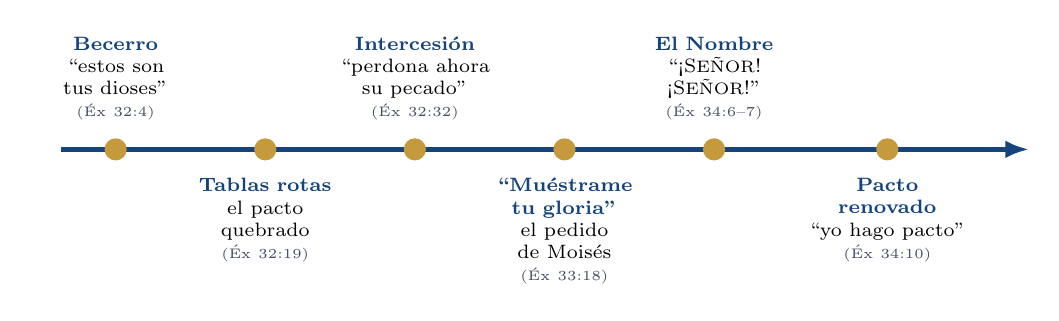
\begin{tikzpicture}[font=\scriptsize]
 \draw[line width=1.6pt,azul,-{Latex[length=3mm]}] (-0.3,0) -- (12.0,0);
 \foreach \x/\t/\b/\r/\pos in {0.4/{Becerro}/{``estos son tus dioses''}/{Éx 32:4}/above,
   2.3/{Tablas rotas}/{el pacto quebrado}/{Éx 32:19}/below,
   4.2/{Intercesión}/{``perdona ahora su pecado''}/{Éx 32:32}/above,
   6.1/{``Muéstrame tu gloria''}/{el pedido de Moisés}/{Éx 33:18}/below,
   8.0/{El Nombre}/{``¡\SENOR! ¡\SENOR!''}/{Éx 34:6--7}/above,
   10.2/{Pacto renovado}/{``yo hago pacto''}/{Éx 34:10}/below}{
  \fill[dorado] (\x,0) circle (4pt);
  \node[\pos=7pt,text width=2.0cm,align=center] at (\x,0) {\textbf{\textcolor{azul}{\t}}\\ \b\\ {\tiny\color{gris}(\r)}};}
\end{tikzpicture}\par\medskip
\small\RaggedRight La revelación más completa del carácter de Dios en el AT llega en el peor momento de Israel: recién ``cambiaron su gloria por la imagen de un buey'' (Sal 106:20). Dios responde mostrando la suya.
\end{frame}

\begin{frame}{``Te ruego que me muestres tu gloria''}
\begin{cita}El entonces dijo: Te ruego que me muestres tu gloria. Y le respondió: Yo haré pasar todo mi bien delante de tu rostro, y proclamaré el nombre de \SENOR{} delante de ti; y tendré misericordia del que tendré misericordia, y seré clemente para con el que seré clemente.\fuente{(Éx 33:18--19, RVR1960)}\end{cita}
\begin{center}\heb{הַרְאֵנִי נָא אֶת־כְּבֹדֶךָ}\\[2pt]\heb{וְחַנֹּתִי אֶת־אֲשֶׁר אָחֹן וְרִחַמְתִּי אֶת־אֲשֶׁר אֲרַחֵם}\end{center}
\scriptsize\renewcommand{\arraystretch}{1.15}
\begin{tabular}{@{}>{\RaggedRight\arraybackslash}p{2.6cm}>{\RaggedRight\arraybackslash}p{1.1cm}>{\RaggedRight\arraybackslash}p{8.0cm}@{}}
\toprule
\heb{כָּבוֹד} \emph{kavod} & \heb{כבד} & ``gloria'': literalmente ``peso''. Moisés pide ver el peso de Dios. \\
\heb{טוּב} \emph{tuv} & \heb{טוב} & ``bien, bondad'': Dios responde a ``gloria'' con ``todo mi bien''. \\
\heb{וְחַנֹּתִי}\ldots{} \heb{אָחֹן} & \heb{חנן} & ``tendré gracia de quien tendré gracia'' (RVR1960 traduce ``tendré misericordia''). \\
\heb{וְרִחַמְתִּי}\ldots{} \heb{אֲרַחֵם} & \heb{רחם} & ``me compadeceré de quien me compadeceré'' (RVR1960: ``seré clemente''). \\
\bottomrule
\end{tabular}\par\smallskip
\precision{la RVR1960 invierte los términos: traduce \emph{janán} como ``misericordia'' y \emph{rajam} como ``clemente''. La fórmula ``\ldots{} de quien \ldots'' (\emph{idem per idem}) afirma la libertad de Dios, como ``Yo soy el que soy'' (Éx 3:14).}
\end{frame}

\begin{frame}{Texto ancla: Éx 34:4--7}
\fotolado{panel_exodo34.jpg}{Elaboración propia: Éx 34:6 en texto hebreo consonántico (BHS).}
\begin{columns}[c,onlytextwidth]
\begin{column}{0.58\textwidth}
\begin{cita}Y Moisés alisó dos tablas de piedra como las primeras; y se levantó de mañana y subió al monte Sinaí\ldots{} Y \SENOR{} descendió en la nube, y estuvo allí con él, proclamando el nombre de \SENOR. Y pasando \SENOR{} por delante de él, proclamó: ¡\SENOR! ¡\SENOR! fuerte, misericordioso y piadoso; tardo para la ira, y grande en misericordia y verdad; que guarda misericordia a millares, que perdona la iniquidad, la rebelión y el pecado, y que de ningún modo tendrá por inocente al malvado; que visita la iniquidad de los padres sobre los hijos y sobre los hijos de los hijos, hasta la tercera y cuarta generación.\fuente{(Éx 34:4--7, RVR1960)}\end{cita}
\end{column}
\begin{column}{0.40\textwidth}\end{column}
\end{columns}
\end{frame}

\begin{frame}{Éx 34:6--7 en hebreo}
\begin{center}
\heb{וַיַּעֲבֹר יְהוָה עַל־פָּנָיו וַיִּקְרָא יְהוָה יְהוָה אֵל רַחוּם וְחַנּוּן}\\[2pt]
\heb{אֶרֶךְ אַפַּיִם וְרַב־חֶסֶד וֶאֱמֶת נֹצֵר חֶסֶד לָאֲלָפִים}\\[2pt]
\heb{נֹשֵׂא עָוֹן וָפֶשַׁע וְחַטָּאָה וְנַקֵּה לֹא יְנַקֶּה}
\end{center}
\renewcommand{\arraystretch}{1.12}\scriptsize
\begin{tabular}{@{}>{\RaggedRight\arraybackslash}p{2.7cm}>{\RaggedRight\arraybackslash}p{1.2cm}>{\RaggedRight\arraybackslash}p{7.9cm}@{}}
\toprule
\textbf{Término} & \textbf{Raíz} & \textbf{Sentido} \\ \midrule
\heb{אֵל} \emph{El} & --- & ``Dios'' (RVR1960: ``fuerte''). \\
\heb{רַחוּם} \emph{rajum} & \heb{רחם} & ``compasivo'', de \emph{réjem}, el vientre materno: la ternura de una madre. \\
\heb{חַנּוּן} \emph{jannun} & \heb{חנן} & ``clemente, lleno de gracia'': se inclina con favor hacia quien no lo merece. \\
\heb{אֶרֶךְ אַפַּיִם} \emph{érej appáyim} & \heb{ארך}, \heb{אנף} & ``largo de narices'': lento para la ira. \\
\heb{רַב־חֶסֶד וֶאֱמֶת} \emph{rav jésed ve'emet} & \heb{חסד}, \heb{אמן} & ``abundante en amor leal y verdad'': los dos pilares del pacto. \\
\heb{נֹצֵר חֶסֶד לָאֲלָפִים} & \heb{נצר} & ``que guarda (vigila) el amor leal para millares''. \\
\heb{נֹשֵׂא עָוֹן} \emph{nosé avón} & \heb{נשׂא} & ``que levanta, carga la iniquidad'': perdonar es cargar con la culpa. \\
\heb{וְנַקֵּה לֹא יְנַקֶּה} & \heb{נקה} & ``y absolver, no absuelve'': el infinitivo absoluto refuerza la negación. \\
\bottomrule
\end{tabular}
\end{frame}

\begin{frame}{La estructura del Nombre}
\centering
\begin{tikzpicture}[font=\scriptsize]
 \node[draw=dorado,line width=1.6pt,fill=azul,text=papiro,rounded corners=3pt,text width=3.0cm,align=center,inner sep=5pt] (n) at (0,0) {\textbf{¡\SENOR! ¡\SENOR!}\\ el Nombre (\heb{יְהוָה})};
 \node[caja,text width=3.2cm,align=center] (a) at (-4.0,-1.9) {\textbf{Lo que es}\\ compasivo, clemente, lento para la ira, abundante en \emph{jésed} y verdad\\ {\tiny\color{gris}(v. 6)}};
 \node[caja,text width=3.2cm,align=center] (b) at (0,-1.9) {\textbf{Lo que hace}\\ guarda \emph{jésed} a millares; carga la iniquidad, la rebelión y el pecado\\ {\tiny\color{gris}(v. 7a)}};
 \node[caja,text width=3.2cm,align=center,fill=gris!15] (c) at (4.0,-1.9) {\textbf{Lo que no hace}\\ no absuelve al culpable impenitente; visita hasta la 3.ª y 4.ª\\ {\tiny\color{gris}(v. 7b)}};
 \foreach \i in {a,b,c}\draw[-{Latex[length=2.5mm]},dorado,line width=1.1pt](n)--(\i);
 \node[text width=11cm,align=center,font=\scriptsize\itshape,text=gris] at (0,-3.4) {Miles de generaciones de \emph{jésed} frente a tres o cuatro de visitación: la misericordia es más grande que el juicio (Stg 2:13).};
\end{tikzpicture}\par\smallskip
\begin{columns}[c,onlytextwidth]
\begin{column}{0.50\textwidth}
\begin{cita}Entonces Moisés, apresurándose, bajó la cabeza hacia el suelo y adoró.\fuente{(Éx 34:8, RVR1960)}\end{cita}
\end{column}
\begin{column}{0.48\textwidth}\scriptsize
Moisés pidió ver la gloria (33:18) y Dios le mostró su \destacar{carácter}. La gloria de Dios es la comunión de sus atributos: la tesis de esta obra.
\end{column}
\end{columns}
\end{frame}

\begin{frame}{La fórmula que recorre la Biblia}
\scriptsize\renewcommand{\arraystretch}{1.18}
\begin{tabular}{@{}>{\RaggedRight\arraybackslash}p{1.9cm}>{\RaggedRight\arraybackslash}p{6.4cm}>{\RaggedRight\arraybackslash}p{3.5cm}@{}}
\toprule
\textbf{Texto} & \textbf{RVR1960} & \textbf{Uso} \\ \midrule
Nm 14:18--19 & ``\SENOR, tardo para la ira y grande en misericordia\ldots{} Perdona ahora la iniquidad de este pueblo según la grandeza de tu misericordia'' & Moisés intercede con la fórmula \\
Sal 86:15 & ``Mas tú, Señor, Dios misericordioso y clemente, lento para la ira, y grande en misericordia y verdad'' & oración personal \\
Sal 103:8 & ``Misericordioso y clemente es \SENOR; lento para la ira, y grande en misericordia'' & alabanza \\
Sal 145:8 & ``Clemente y misericordioso es \SENOR, lento para la ira, y grande en misericordia'' & alabanza (acróstico) \\
Jl 2:13 & ``porque misericordioso es y clemente, tardo para la ira y grande en misericordia'' & llamado al arrepentimiento \\
Jon 4:2 & ``sabía yo que tú eres Dios clemente y piadoso, tardo en enojarte, y de grande misericordia'' & queja del profeta \\
Nah 1:3 & ``\SENOR{} es tardo para la ira\ldots{} y no tendrá por inocente al culpable'' & juicio de Nínive \\
\bottomrule
\end{tabular}\par\medskip
\small\RaggedRight Israel no inventó un concepto nuevo de Dios en cada época: \destacar{repitió el Nombre} que Dios proclamó en el Sinaí. Es el ``credo'' más citado del AT.
\end{frame}

% ------------------------------------------------------------------
\section{La palabra}

\begin{frame}{El espectro completo: hebreo y arameo}
\scriptsize\renewcommand{\arraystretch}{1.13}
\begin{tabular}{@{}>{\RaggedRight\arraybackslash}p{1.0cm}>{\RaggedRight\arraybackslash}p{3.6cm}>{\RaggedRight\arraybackslash}p{3.7cm}>{\RaggedRight\arraybackslash}p{3.3cm}@{}}
\toprule
\textbf{Raíz} & \textbf{Términos} & \textbf{Imagen y sentido} & \textbf{Textos} \\ \midrule
\heb{חסד} & \heb{חֶסֶד} \emph{jésed}; \heb{חָסִיד} \emph{jasid} ``misericordioso''; \heb{הִתְחַסֵּד} \emph{hitjassed} ``mostrarse misericordioso'' & lealtad de pacto; el \emph{jasid} es el que vive en \emph{jésed} & Éx 34:6; Sal 136; Sal 18:25; Jer 3:12; Mi 7:2 \\
\heb{רחם} & \heb{רַחֲמִים} \emph{rajamím}; \heb{רָחַם} \emph{rajam}; \heb{רַחוּם} \emph{rajum} & el vientre (\emph{réjem}): ternura de entrañas & Sal 103:13; Jer 31:20; Os 2:23 \\
\heb{חנן} & \heb{חָנַן} \emph{janán}; \heb{חַנּוּן} \emph{jannun}; \heb{חֵן} \emph{jen}; \heb{תְּחִנָּה} \emph{tejinná}; \heb{תַּחֲנוּנִים} \emph{tajanunim} & inclinarse con favor; la gracia que se \emph{suplica} & Sal 86:3; Pr 14:21; Jos 11:20; Esd 9:8; Jer 31:9 \\
\heb{חמל} & \heb{חָמַל} \emph{jamal}; \heb{חֶמְלָה} \emph{jemlá} & perdonar la vida, no destruir & Gn 19:16; Mal 3:17; Ez 5:11 \\
\heb{חוס} & \heb{חוּס} \emph{jus} & el ojo que ``tiene lástima'' & Sal 72:13; Jon 4:11; Ez 5:11 \\
\heb{נחם} & \heb{נִחַם} \emph{nijam} (nifal) & conmoverse hasta cambiar el curso & Jue 2:18 \\
\heb{טוב} & \heb{טוֹב־עַיִן} \emph{tov ayin} & ``bueno de ojo'': el generoso & Pr 22:9 \\
arameo & \heb{רַחֲמִין} \emph{rajamín}; \heb{מִחַן} \emph{mijan} (de \heb{חֲנַן}) & compasión; hacer gracia al oprimido & Dn 2:18; 4:27 \\
\bottomrule
\end{tabular}\par\smallskip
\precision{\emph{nijam} suele traducirse ``arrepentirse'' (de Dios: cambiar el curso); solo en Jue 2:18 la RVR1960 lo vierte ``era movido a misericordia''.}
\end{frame}

\begin{frame}{El espectro completo: griego}
\scriptsize\renewcommand{\arraystretch}{1.13}
\begin{tabular}{@{}>{\RaggedRight\arraybackslash}p{3.3cm}>{\RaggedRight\arraybackslash}p{3.8cm}>{\RaggedRight\arraybackslash}p{1.0cm}>{\RaggedRight\arraybackslash}p{3.5cm}@{}}
\toprule
\textbf{Término} & \textbf{Sentido} & \textbf{Vv.} & \textbf{Textos} \\ \midrule
\grc{ἔλεος}, \grc{ἐλεέω} & misericordia; tener misericordia (LXX: \emph{jésed}) & 26; 28 & Mt 9:13; Ro 9:15; Ef 2:4 \\
\grc{ἐλεήμων} & misericordioso & 2 & Mt 5:7; He 2:17 \\
\grc{ἀνέλεος}, \grc{ἀνελεήμων} & sin misericordia & 1; 1 & Stg 2:13; Ro 1:31 \\
\grc{οἰκτιρμός}, \grc{οἰκτίρμων} & compasión; compasivo (LXX: \emph{rajamím}, \emph{rajum}) & 4; 2 & Ro 12:1; 2 Co 1:3; Lc 6:36 \\
\grc{σπλαγχνίζομαι} & conmoverse en las entrañas & 5 & Mt 18:27; Lc 10:33; 15:20 \\
\grc{σπλάγχνα} & ``entrañas'': ``entrañable misericordia'' & 3 & Lc 1:78; Flp 2:1; Col 3:12 \\
\grc{εὔσπλαγχνος} & ``de buenas entrañas'' & 2 & Ef 4:32; 1 P 3:8 \\
\grc{πολύσπλαγχνος} & ``de muchas entrañas'' & 1 & Stg 5:11 \\
\grc{ὅσιος} & \grc{τὰ ὅσια Δαυίδ}: las lealtades a David & 1 & Hch 13:34 (= Is 55:3 \emph{jasdé David}) \\
\bottomrule
\end{tabular}\par\smallskip
\precision{dos casos especiales: en Mt 21:41 ``sin misericordia'' traduce \grc{κακῶς}, ``malamente''; en Tit 1:4 ``misericordia'' (\grc{ἔλεος}) está en el Texto Recibido, no en NA28.}
\end{frame}

\begin{frame}{Las palabras menores: hebreo}
\begin{columns}[t,onlytextwidth]
\begin{column}{0.49\textwidth}
\begin{cita}Faltó el misericordioso de la tierra, y ninguno hay recto entre los hombres.\fuente{(Mi 7:2, RVR1960)}\end{cita}
\scriptsize\heb{אָבַד חָסִיד מִן־הָאָרֶץ}: el \emph{jasid} es el hombre de \emph{jésed}. Dios mismo dice: ``misericordioso (\heb{חָסִיד}) soy yo'' (Jer 3:12).
\begin{cita}Y ahora por un breve momento ha habido misericordia de parte de \SENOR{} nuestro Dios, para hacer que nos quedase un remanente libre.\fuente{(Esd 9:8, RVR1960)}\end{cita}
\scriptsize\heb{תְחִנָּה} (\emph{tejinná}): la gracia como respuesta a la súplica.
\end{column}
\begin{column}{0.49\textwidth}
\begin{cita}porque \SENOR{} era movido a misericordia por sus gemidos a causa de los que los oprimían y afligían.\fuente{(Jue 2:18, RVR1960)}\end{cita}
\scriptsize\heb{כִּי יִנָּחֵם יְהוָה מִנַּאֲקָתָם}: los gemidos de Israel conmueven a Dios.
\begin{cita}El ojo misericordioso será bendito, Porque dio de su pan al indigente.\fuente{(Pr 22:9, RVR1960)}\end{cita}
\scriptsize\heb{טוֹב־עַיִן}: ``bueno de ojo''. La misericordia mira bien al necesitado.
\end{column}
\end{columns}
\end{frame}

\begin{frame}{Las palabras menores: griego}
\begin{columns}[t,onlytextwidth]
\begin{column}{0.49\textwidth}
\begin{cita}Os daré las misericordias fieles de David.\fuente{(Hch 13:34, RVR1960)}\end{cita}
\scriptsize Pablo, en Antioquía de Pisidia, cita Is 55:3 (\heb{חַסְדֵי דָוִד הַנֶּאֱמָנִים}) con la LXX: \grc{τὰ ὅσια Δαυὶδ τὰ πιστά}, y lo aplica a la resurrección de Cristo. El \emph{jésed} prometido a David se cumple en el Resucitado.
\begin{cita}Por lo cual debía ser en todo semejante a sus hermanos, para venir a ser misericordioso y fiel sumo sacerdote.\fuente{(He 2:17, RVR1960)}\end{cita}
\scriptsize\grc{ἐλεήμων καὶ πιστός}: ``misericordioso y fiel'', el par \emph{jésed ve'emet} hecho persona.
\end{column}
\begin{column}{0.49\textwidth}
\begin{cita}el Señor es muy misericordioso y compasivo.\fuente{(Stg 5:11, RVR1960)}\end{cita}
\scriptsize\grc{πολύσπλαγχνός ἐστιν ὁ κύριος καὶ οἰκτίρμων}: ``de muchas entrañas y compasivo'', eco de Éx 34:6.
\begin{cita}Antes sed benignos unos con otros, misericordiosos, perdonándoos unos a otros, como Dios también os perdonó a vosotros en Cristo.\fuente{(Ef 4:32, RVR1960)}\end{cita}
\scriptsize\grc{εὔσπλαγχνοι}: ``de buenas entrañas''.
\end{column}
\end{columns}
\precision{Hechos y Hebreos no son cartas de Pablo; Hch 13:34 recoge un discurso suyo según Lucas.}
\end{frame}

\begin{frame}{Cuatro columnas de la misericordia}
\centering
\begin{tikzpicture}
 \fill[azul] (-0.4,3.0) -- (11.4,3.0) -- (5.5,4.0) -- cycle;
 \draw[dorado,line width=1.4pt] (-0.4,3.0) -- (11.4,3.0) -- (5.5,4.0) -- cycle;
 \node[text=papiro,font=\small\bfseries] at (5.5,3.35) {LA MISERICORDIA};
 \fill[dorado] (-0.4,-0.25) rectangle (11.4,-0.05);
 \foreach \x/\h/\t/\s in {0.8/{חָנַן}/{janán}/{gracia, favor inmerecido},
   3.95/{חֶסֶד}/{jésed}/{amor leal del pacto},
   7.05/{רַחֲמִים}/{rajamím}/{compasión desde las entrañas},
   10.2/{חָמַל}/{jamal}/{perdonar la vida; clemencia}}{
  \fill[papiro,opacity=0.9] (\x-1.1,0) rectangle (\x+1.1,2.9);
  \draw[azul,line width=0.8pt] (\x-1.1,0) rectangle (\x+1.1,2.9);
  \foreach \k in {-0.7,-0.35,0,0.35,0.7}\draw[dorado!60,line width=0.5pt] (\x+\k,0.1) -- (\x+\k,0.55);
  \node[font=\large] at (\x,2.3) {\heb{\h}};
  \node[font=\small\bfseries\itshape,text=azul] at (\x,1.65) {\t};
  \node[font=\scriptsize,text width=1.9cm,align=center] at (\x,1.05) {\s};}
\end{tikzpicture}\par\medskip
\small\RaggedRight De todo el espectro, las cuatro palabras de tu material son las columnas: sostienen un mismo techo. Ninguna basta sola; juntas muestran cómo Dios se acerca al que no merece, al que pertenece a su pacto, al que sufre y al que debería morir.
\end{frame}

\begin{frame}{\emph{Janán}: gracia, favor inmerecido}
\begin{columns}[t,onlytextwidth]
\begin{column}{0.50\textwidth}
\begin{cita}\SENOR{} haga resplandecer su rostro sobre ti, y tenga de ti misericordia.\fuente{(Nm 6:25, RVR1960)}\end{cita}
\begin{center}\heb{יָאֵר יְהוָה פָּנָיו אֵלֶיךָ וִיחֻנֶּךָּ}\end{center}
\begin{cita}Ten misericordia de mí, oh Señor; Porque a ti clamo todo el día.\fuente{(Sal 86:3, RVR1960)}\end{cita}
\begin{center}\heb{חָנֵּנִי אֲדֹנָי כִּי אֵלֶיךָ אֶקְרָא כָּל־הַיּוֹם}\end{center}
\end{column}
\begin{column}{0.48\textwidth}\scriptsize
\heb{חָנַן} (\emph{janán}; Strong H2603): ``inclinarse en bondad hacia un inferior''. De la misma raíz vienen \heb{חֵן} (\emph{jen}, ``gracia''), \heb{חַנּוּן} (\emph{jannun}, ``clemente'') y \heb{תְּחִנָּה} (\emph{tejinná}, ``súplica''). La forma reflexiva significa \emph{implorar}: pedir gracia.\par\medskip
\small
\begin{itemize}
\item En la bendición sacerdotal, la gracia va unida al \destacar{rostro} de Dios que resplandece.
\item En el Salmo, el que no tiene derechos \destacar{clama todo el día}.
\item ``Tendré gracia de quien tendré gracia'' (Éx 33:19): es un don libre.
\end{itemize}
\end{column}
\end{columns}
\end{frame}

\begin{frame}{\emph{Janán}: ``¿qué a ti?''}
\begin{columns}[t,onlytextwidth]
\begin{column}{0.49\textwidth}
\begin{cita}Cuando Pedro le vio, dijo a Jesús: Señor, ¿y qué de éste? Jesús le dijo: Si quiero que él quede hasta que yo venga, ¿qué a ti? Sígueme tú.\fuente{(Jn 21:21--22, RVR1960)}\end{cita}
\small Éx 33:19 dice ``tendré gracia \destacar{de quien} tendré gracia''; Jesús le dice a Pedro ``¿qué a ti?''. La gracia de Dios no se administra con nuestro criterio.\par\smallskip
\precision{la conexión entre Éx 33:19 y Jn 21:22 es tuya, una lectura propia.}
\end{column}
\begin{column}{0.49\textwidth}
\begin{cita}Entonces aquel siervo, postrado, le suplicaba, diciendo: Señor, ten paciencia conmigo, y yo te lo pagaré todo. El señor de aquel siervo, movido a misericordia, le soltó y le perdonó la deuda.\fuente{(Mt 18:26--27, RVR1960)}\end{cita}
\scriptsize Diez mil talentos (18:24) era una deuda impagable. El siervo implora (lo que el hebreo diría \emph{hitjanén}) y el rey le perdona todo: gracia pura. \grc{σπλαγχνισθείς}: ``conmovido en las entrañas''.
\end{column}
\end{columns}
\end{frame}

\begin{frame}{\emph{Rajamím}: entrañas}
\fotolado{panel_jeremias31.jpg}{Elaboración propia: Jer 31:20 en texto hebreo consonántico (BHS).}
\begin{columns}[c,onlytextwidth]
\begin{column}{0.58\textwidth}
\begin{cita}Como el padre se compadece de los hijos, Se compadece \SENOR{} de los que le temen.\fuente{(Sal 103:13, RVR1960)}\end{cita}
\begin{center}\heb{כְּרַחֵם אָב עַל־בָּנִים רִחַם יְהוָה עַל־יְרֵאָיו}\end{center}
\scriptsize
\heb{רֶחֶם} (\emph{réjem}): ``vientre, matriz'' (H7358). \heb{רַחֲמִים} (\emph{rajamím}) es su plural: ``entrañas'', y de ahí ``compasión''. Es el amor que se siente en el cuerpo, como el de una madre por el hijo que llevó dentro (1~R 3:26: ``sus entrañas se le conmovieron por su hijo'').\par\smallskip
\small El Salmo aplica la imagen a un \destacar{padre}: la ternura de Dios reúne la de la madre y la del padre.
\end{column}
\begin{column}{0.40\textwidth}\end{column}
\end{columns}
\end{frame}

\begin{frame}{\emph{Rajamím}: Efraín, hijo precioso}
\begin{cita}Escuchando, he oído a Efraín que se lamentaba: Me azotaste, y fui castigado como novillo indómito; conviérteme, y seré convertido, porque tú eres \SENOR{} mi Dios. Porque después que me aparté tuve arrepentimiento\ldots{} ¿No es Efraín hijo precioso para mí? ¿no es niño en quien me deleito? pues desde que hablé de él, me he acordado de él constantemente. Por eso mis entrañas se conmovieron por él; ciertamente tendré de él misericordia, dice \SENOR.\fuente{(Jer 31:18--20, RVR1960)}\end{cita}
\begin{center}\heb{עַל־כֵּן הָמוּ מֵעַי לוֹ רַחֵם אֲרַחֲמֶנּוּ נְאֻם־יְהוָה}\end{center}
\scriptsize\renewcommand{\arraystretch}{1.12}
\begin{tabular}{@{}>{\RaggedRight\arraybackslash}p{2.6cm}>{\RaggedRight\arraybackslash}p{9.2cm}@{}}
\toprule
\heb{הָמוּ מֵעַי} \emph{hamú me'ay} & ``mis entrañas se agitaron'' (\heb{המה}, ``bramar, conmoverse''). \\
\heb{רַחֵם אֲרַחֲמֶנּוּ} \emph{rajem arajamennu} & ``compadecer, me compadeceré de él'': el infinitivo absoluto intensifica (RVR1960: ``ciertamente''). \\
\bottomrule
\end{tabular}
\end{frame}

\begin{frame}{\emph{Rajamím} en Jesús}
\begin{columns}[t,onlytextwidth]
\begin{column}{0.49\textwidth}
\begin{cita}Y levantándose, vino a su padre. Y cuando aún estaba lejos, lo vio su padre, y fue movido a misericordia, y corrió, y se echó sobre su cuello, y le besó.\fuente{(Lc 15:20, RVR1960)}\end{cita}
\scriptsize\grc{ἐσπλαγχνίσθη} (\emph{esplanjnísthē}), de \grc{σπλάγχνα}, ``entrañas'': el equivalente griego de \emph{rajamím}. El padre de la parábola actúa como el Dios de Jer 31:20 con Efraín.
\end{column}
\begin{column}{0.49\textwidth}
\begin{cita}Jesús entonces, al verla llorando, y a los judíos que la acompañaban, también llorando, se estremeció en espíritu y se conmovió\ldots{} Jesús lloró.\fuente{(Jn 11:33, 35, RVR1960)}\end{cita}
\scriptsize\grc{ἐνεβριμήσατο} ``se estremeció'' y \grc{ἐτάραξεν ἑαυτόν} ``se turbó''; \grc{ἐδάκρυσεν} ``lloró''.\par\smallskip
\precision{Jn 11:33 no usa \grc{σπλαγχνίζομαι}; muestra la compasión de Jesús con otros verbos. El verbo de las entrañas aparece en los evangelios sinópticos (Mt 9:36; 14:14; Lc 7:13).}
\end{column}
\end{columns}
\end{frame}

\begin{frame}{\emph{Jamal}: perdonar la vida, levantar}
\begin{columns}[t,onlytextwidth]
\begin{column}{0.50\textwidth}
\begin{cita}Y deteniéndose él, los varones asieron de su mano, y de la mano de su mujer y de las manos de sus dos hijas, según la misericordia de \SENOR{} para con él; y lo sacaron y lo pusieron fuera de la ciudad.\fuente{(Gn 19:16, RVR1960)}\end{cita}
\begin{center}\heb{בְּחֶמְלַת יְהוָה עָלָיו}\end{center}
\begin{cita}Y serán para mí especial tesoro, ha dicho \SENOR{} de los ejércitos\ldots{} y los perdonaré, como el hombre que perdona a su hijo que le sirve.\fuente{(Mal 3:17, RVR1960)}\end{cita}
\begin{center}\heb{וְחָמַלְתִּי עֲלֵיהֶם כַּאֲשֶׁר יַחְמֹל אִישׁ עַל־בְּנוֹ}\end{center}
\end{column}
\begin{column}{0.48\textwidth}\scriptsize
\heb{חָמַל} (\emph{jamal}; H2550): ``tener compasión'' y, por implicación, ``librar, perdonar la vida, no destruir''. Es la misericordia que \destacar{saca} del lugar del juicio.\par\medskip
\small
\begin{itemize}
\item Lot \destacar{se demoraba}; la misericordia lo toma de la mano y lo saca de Sodoma.
\item En Malaquías, Dios ``perdona'' a los suyos como un padre a su hijo: los preserva en el día del juicio.
\end{itemize}
\end{column}
\end{columns}
\end{frame}

\begin{frame}{Jonás: la piedad por Nínive}
\begin{cita}Y dijo \SENOR: Tuviste tú lástima de la calabacera, en la cual no trabajaste, ni tú la hiciste crecer; que en espacio de una noche nació, y en espacio de otra noche pereció. ¿Y no tendré yo piedad de Nínive, aquella gran ciudad donde hay más de ciento veinte mil personas que no saben discernir entre su mano derecha y su mano izquierda, y muchos animales?\fuente{(Jon 4:10--11, RVR1960)}\end{cita}
\begin{center}\heb{וַאֲנִי לֹא אָחוּס עַל־נִינְוֵה הָעִיר הַגְּדוֹלָה}\end{center}
\scriptsize\renewcommand{\arraystretch}{1.12}
\begin{tabular}{@{}>{\RaggedRight\arraybackslash}p{2.2cm}>{\RaggedRight\arraybackslash}p{9.6cm}@{}}
\toprule
\heb{חוּס} \emph{jus} & ``tener lástima, perdonar la vida'' (H2347): Jonás ``tuvo lástima'' de una planta; Dios, de una ciudad entera, hasta de sus animales. \\
\bottomrule
\end{tabular}\par\smallskip
\precision{Jonás 4:10--11 no usa \emph{jamal} sino \emph{jus}, un sinónimo cercano. El libro termina con una pregunta sin respuesta: la deja al lector.}
\end{frame}

\begin{frame}{\emph{Jésed}: amor leal del pacto}
\begin{columns}[t,onlytextwidth]
\begin{column}{0.50\textwidth}
\begin{cita}Por la misericordia de \SENOR{} no hemos sido consumidos, porque nunca decayeron sus misericordias. Nuevas son cada mañana; grande es tu fidelidad.\fuente{(Lam 3:22--23, RVR1960)}\end{cita}
\begin{center}\heb{חַסְדֵי יְהוָה כִּי לֹא־תָמְנוּ כִּי לֹא־כָלוּ רַחֲמָיו}\end{center}
\begin{cita}Todas las sendas de \SENOR{} son misericordia y verdad, Para los que guardan su pacto y sus testimonios.\fuente{(Sal 25:10, RVR1960)}\end{cita}
\end{column}
\begin{column}{0.48\textwidth}\scriptsize
\heb{חֶסֶד} (\emph{jésed}; H2617): bondad leal, amor que se mantiene por compromiso. Es la palabra del \destacar{pacto} (\heb{בְּרִית}, \emph{berit}): la lealtad que Dios jura y cumple.\par\smallskip
En Lam 3:22 aparecen juntos \emph{jasdé} (``las misericordias'', plural de \emph{jésed}) y \emph{rajamav} (``sus compasiones''). Lamentaciones 3 es un acróstico triple; este verso está en el centro del libro, entre las ruinas de Jerusalén.\par\smallskip
\precision{\emph{jésed} no tiene equivalente exacto en español; la RVR1960 lo traduce ``misericordia'' 205 veces, pero también ``bondad'', ``benignidad'', ``favor'' (Strong H2617).}
\end{column}
\end{columns}
\end{frame}

\begin{frame}{\emph{Jésed}: ``misericordia quiero''}
\begin{columns}[t,onlytextwidth]
\begin{column}{0.49\textwidth}
\begin{cita}Porque misericordia quiero, y no sacrificio, y conocimiento de Dios más que holocaustos.\fuente{(Os 6:6, RVR1960)}\end{cita}
\begin{center}\heb{כִּי חֶסֶד חָפַצְתִּי וְלֹא־זָבַח}\end{center}
\scriptsize En Oseas, \emph{jésed} es lo que Dios espera de Israel: la lealtad del pacto vivida, no solo el rito. El verso anterior se queja: ``la piedad (\emph{jésed}) vuestra es como nube de la mañana'' (Os 6:4).
\end{column}
\begin{column}{0.49\textwidth}
\begin{cita}Id, pues, y aprended lo que significa: Misericordia quiero, y no sacrificio. Porque no he venido a llamar a justos, sino a pecadores, al arrepentimiento.\fuente{(Mt 9:13, RVR1960)}\end{cita}
\scriptsize Jesús cita Os 6:6 dos veces (Mt 9:13; 12:7). La LXX traduce \emph{jésed} con \grc{ἔλεος}: \grc{διότι ἔλεος θέλω καὶ οὐ θυσίαν}. El puente es directo: \emph{jésed} $\rightarrow$ \emph{éleos}.
\end{column}
\end{columns}
\end{frame}

\begin{frame}{Del hebreo a Pablo}
\centering
\begin{tikzpicture}[font=\scriptsize,node distance=0.7cm]
 \node[caja,text width=3.1cm,align=center] (h) {\textbf{Hebreo (Éx 34:6)}\\ \heb{רַחוּם} \emph{rajum}\\ \heb{חַנּוּן} \emph{jannun}\\ \heb{רַב־חֶסֶד} \emph{rav jésed}};
 \node[caja,text width=3.1cm,align=center,right=of h] (l) {\textbf{Septuaginta}\\ \grc{οἰκτίρμων}\\ \grc{ἐλεήμων}\\ \grc{πολυέλεος}};
 \node[caja,text width=3.1cm,align=center,right=of l] (p) {\textbf{Pablo}\\ \grc{πατὴρ τῶν οἰκτιρμῶν} (2 Co 1:3)\\ \grc{πλούσιος ἐν ἐλέει} (Ef 2:4)\\ \grc{ἐλεήσω ὃν ἂν ἐλεῶ} (Ro 9:15)};
 \draw[-{Latex[length=2.5mm]},dorado,line width=1.2pt] (h)--(l);
 \draw[-{Latex[length=2.5mm]},dorado,line width=1.2pt] (l)--(p);
 \node[below=0.35cm of l,text width=11cm,align=center,font=\scriptsize\itshape,text=gris] {La LXX traduce el Nombre de Éx 34:6 con \emph{oiktírmōn}, \emph{eleēmōn} y \emph{polyéleos}; Pablo hereda ese vocabulario.};
\end{tikzpicture}\par\medskip
\scriptsize\renewcommand{\arraystretch}{1.15}
\begin{tabular}{@{}>{\RaggedRight\arraybackslash}p{2.6cm}>{\RaggedRight\arraybackslash}p{9.2cm}@{}}
\toprule
\grc{ἔλεος} \emph{éleos} & compasión activa ante la miseria; en la LXX traduce casi siempre \emph{jésed} (BDAG). \\
\grc{οἰκτιρμός} \emph{oiktirmós} & compasión, piedad que se conmueve; en la LXX traduce \emph{rajamím}. \\
\grc{σπλαγχνίζομαι} \emph{splanjnízomai} & conmoverse en las entrañas; solo en los evangelios. \\
\bottomrule
\end{tabular}
\end{frame}

% ------------------------------------------------------------------
\section{El Nombre}

\begin{frame}{``Dios misericordioso es el \SENOR{} tu Dios''}
\begin{columns}[c,onlytextwidth]
\begin{column}{0.50\textwidth}
\begin{cita}porque Dios misericordioso es \SENOR{} tu Dios; no te dejará, ni te destruirá, ni se olvidará del pacto que les juró a tus padres.\fuente{(Dt 4:31, RVR1960)}\end{cita}
\begin{center}\small\heb{כִּי אֵל רַחוּם יְהוָה אֱלֹהֶיךָ}\\ \heb{לֹא יַרְפְּךָ וְלֹא יַשְׁחִיתֶךָ}\end{center}
\small Moisés anuncia el destierro (Dt 4:27) y el regreso (4:29--30): el Nombre \emph{El rajum} \destacar{garantiza el regreso}.
\end{column}
\begin{column}{0.48\textwidth}\scriptsize
\renewcommand{\arraystretch}{1.2}
\begin{tabular}{@{}>{\RaggedRight\arraybackslash}p{1.9cm}>{\RaggedRight\arraybackslash}p{3.8cm}@{}}
\toprule
\textbf{Término} & \textbf{Sentido} \\ \midrule
\heb{אֵל רַחוּם} \emph{El rajum} & ``Dios compasivo'': el primer adjetivo de Éx 34:6 hecho título. \\
\heb{לֹא יַרְפְּךָ} \emph{lo yarpeja} & ``no aflojará'' su mano. \\
\heb{וְלֹא יִשְׁכַּח} \emph{velo yishkaj} & ``ni se olvidará'' del pacto. \\
\bottomrule
\end{tabular}\par\medskip
\small Israel ora con este Nombre: Neh 9:31; Sal 145:8; y Jonás, para quejarse: ``sabía yo que tú eres Dios clemente y piadoso'' (Jon 4:2).
\end{column}
\end{columns}
\end{frame}

\begin{frame}{``Cuando tengo misericordia de mi mundo''}
\begin{columns}[c,onlytextwidth]
\begin{column}{0.46\textwidth}
\begin{center}\heb{וכשאני מרחם על עולמי אני נקרא ה׳}\end{center}
\small ``Cuando tengo misericordia de mi mundo, soy llamado \SENOR{}'' (\emph{Shemot Rabá} 3:6).\par\smallskip
\precision{lectura rabínica (R. Abbá bar Memel). El tetragrama, medida de misericordia; \emph{Elohim}, medida del juicio (Rashi a Gn 1:1).}\par\medskip
\small Pablo hace de la misericordia el nombre del Padre: \grc{ὁ πατὴρ τῶν οἰκτιρμῶν} (2~Co 1:3; LXX \emph{rajamím}) y \grc{πλούσιος ἐν ἐλέει} (Ef 2:4; LXX \emph{jésed}).
\end{column}
\begin{column}{0.52\textwidth}\scriptsize
\renewcommand{\arraystretch}{1.15}
\begin{tabular}{@{}>{\RaggedRight\arraybackslash}p{2.6cm}>{\RaggedRight\arraybackslash}p{2.2cm}>{\RaggedRight\arraybackslash}p{1.6cm}@{}}
\toprule
\textbf{Nombre} & \textbf{Original} & \textbf{Texto} \\ \midrule
Fuerte, misericordioso y piadoso & \heb{אֵל רַחוּם וְחַנּוּן} & Éx 34:6 \\
Dios misericordioso & \heb{אֵל רַחוּם} & Dt 4:31 \\
Dios clemente y misericordioso & \heb{אֵל־חַנּוּן וְרַחוּם} & Neh 9:31 \\
Padre de misericordias & \grc{ὁ πατὴρ τῶν οἰκτιρμῶν} & 2~Co 1:3 \\
Rico en misericordia & \grc{πλούσιος ἐν ἐλέει} & Ef 2:4 \\
\emph{HaRajamán} & \heb{הָרַחֲמָן} & Liturgia \\
\bottomrule
\end{tabular}
\end{column}
\end{columns}
\end{frame}

% ------------------------------------------------------------------
\section{Definición}

\begin{frame}{Qué es la misericordia de Dios}
\begin{tcolorbox}[colback=papiro,colframe=azul,boxrule=1pt,arc=3pt,fonttitle=\bfseries\small,title=Definición]
\small La misericordia de Dios es la perfección eterna por la cual Dios, \destacar{movido desde sus entrañas y fiel a su pacto}, se inclina hacia el miserable y el culpable para aliviarlo, perdonarlo y levantarlo, sin dejar de ser justo (Éx 34:6--7).
\end{tcolorbox}
\scriptsize\renewcommand{\arraystretch}{1.2}
\begin{tabular}{@{}>{\RaggedRight\arraybackslash}p{2.4cm}>{\RaggedRight\arraybackslash}p{5.6cm}>{\RaggedRight\arraybackslash}p{3.6cm}@{}}
\toprule
\textbf{Rasgo} & \textbf{Qué afirma} & \textbf{Textos} \\ \midrule
Libre (\emph{janán}) & no se merece ni se exige & Éx 33:19; Ro 9:15 \\
Leal (\emph{jésed}) & se apoya en el pacto & Sal 25:10; Lam 3:22 \\
Tierna (\emph{rajamím}) & nace de las entrañas & Sal 103:13; Jer 31:20 \\
Que salva (\emph{jamal}) & saca del lugar del juicio & Gn 19:16; Mal 3:17 \\
Justa & no absuelve al impenitente & Éx 34:7; Nm 14:18 \\
\bottomrule
\end{tabular}\par\smallskip
\begin{center}\footnotesize
\begin{tabular}{ll}
\textbf{Clasificación:} & Relación con el ser humano (¿cómo se revela?)\\
\textbf{Tipo:} & \destacar{comunicable}: ``Sed, pues, misericordiosos'' (Lc 6:36)\\
\end{tabular}
\end{center}
\end{frame}

\begin{frame}{Misericordia y gracia}
\begin{columns}[c,onlytextwidth]
\begin{column}{0.50\textwidth}\small
\begin{itemize}
\item Pink: la misericordia nace de la bondad de Dios y es ``la pronta inclinación de Dios a aliviar la miseria de las criaturas caídas''; por eso \destacar{presupone el pecado} (Pink, 2020, cap. 14).
\item Los ángeles que no cayeron reciben \destacar{gracia} (fueron elegidos y preservados), pero no misericordia: nunca la necesitaron.
\item La gracia mira al \emph{culpable} que no merece; la misericordia mira al \emph{miserable} que sufre.
\end{itemize}
\end{column}
\begin{column}{0.48\textwidth}
\centering
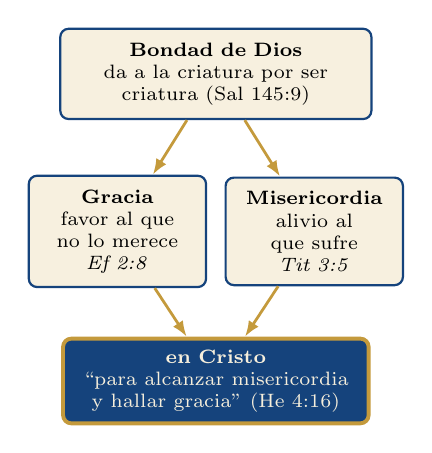
\begin{tikzpicture}[font=\scriptsize]
 \node[caja,text width=3.6cm,align=center] (b) at (0,2.0) {\textbf{Bondad de Dios}\\ da a la criatura por ser criatura (Sal 145:9)};
 \node[caja,text width=1.9cm,align=center] (g) at (-1.25,0) {\textbf{Gracia}\\ favor al que no lo merece\\ \emph{Ef 2:8}};
 \node[caja,text width=1.9cm,align=center] (m) at (1.25,0) {\textbf{Misericordia}\\ alivio al que sufre\\ \emph{Tit 3:5}};
 \node[draw=dorado,line width=1.4pt,fill=azul,text=papiro,rounded corners=3pt,text width=3.6cm,align=center,inner sep=4pt] (c) at (0,-1.9) {\textbf{en Cristo}\\ ``para alcanzar misericordia y hallar gracia'' (He 4:16)};
 \draw[-{Latex[length=2mm]},dorado,line width=1pt](b)--(g); \draw[-{Latex[length=2mm]},dorado,line width=1pt](b)--(m);
 \draw[-{Latex[length=2mm]},dorado,line width=1pt](g)--(c); \draw[-{Latex[length=2mm]},dorado,line width=1pt](m)--(c);
\end{tikzpicture}
\end{column}
\end{columns}
\end{frame}

\begin{frame}{Siempre juntas: \emph{jésed} y \emph{emet}}
\begin{columns}[c,onlytextwidth]
\begin{column}{0.48\textwidth}
\begin{cita}La misericordia y la verdad se encontraron; La justicia y la paz se besaron.\fuente{(Sal 85:10 [85:11], RVR1960)}\end{cita}
\begin{center}\heb{חֶסֶד־וֶאֱמֶת נִפְגָּשׁוּ}\\ \heb{צֶדֶק וְשָׁלוֹם נָשָׁקוּ}\end{center}
\scriptsize\heb{אֱמֶת} (\emph{emet}), de \heb{אמן}: ``firmeza, fidelidad, verdad''. Es lo que hace confiable el \emph{jésed}. El par aparece desde Éx 34:6 (\emph{rav jésed ve'emet}).
\end{column}
\begin{column}{0.50\textwidth}
\scriptsize\renewcommand{\arraystretch}{1.15}
\begin{tabular}{@{}>{\RaggedRight\arraybackslash}p{1.5cm}>{\RaggedRight\arraybackslash}p{4.3cm}@{}}
\toprule
Éx 34:6 & ``grande en misericordia y verdad'' \\
Sal 25:10 & ``sendas\ldots{} misericordia y verdad'' \\
Sal 85:10 & ``la misericordia y la verdad se encontraron'' \\
Mi 7:20 & ``cumplirás la verdad a Jacob, y a Abraham la misericordia'' \\
Jn 1:14 & ``lleno de gracia y de verdad'' \\
\bottomrule
\end{tabular}\par\medskip
\small Misericordia sin verdad sería sentimentalismo; verdad sin misericordia, dureza. En Dios van \destacar{siempre juntas}.\par\smallskip
\precision{leer Jn 1:14 como eco de \emph{rav jésed ve'emet} es una lectura extendida (Carson, 1991).}
\end{column}
\end{columns}
\end{frame}

% ------------------------------------------------------------------
\section{Pink}

\begin{frame}{Teología: la exposición de Pink}
\begin{columns}[t,onlytextwidth]
\begin{column}{0.55\textwidth}\small
Recorrido de Pink (2020, caps. 14--15):
\begin{enumerate}
\item La misericordia se origina en la bondad de Dios y presupone la miseria del pecado.
\item Tres niveles: \destacar{general} (toda la creación, Sal 145:9), \destacar{especial} (todos los hombres, Mt 5:45) y \destacar{soberana} (los herederos de la salvación, por el Mediador).
\item Dios nunca deja de ser misericordioso, pero el ejercicio de su misericordia lo regula su voluntad (Ro 9:15).
\item Es presunción contar con ella y seguir pecando (Éx 34:7).
\item Su ``tierna misericordia'' (\emph{jésed}) va unida a su verdad y a su pacto (Sal 89:33--34).
\end{enumerate}
\end{column}
\begin{column}{0.43\textwidth}
\begin{cita}Alabad a \SENOR, porque él es bueno; porque para siempre es su misericordia.\fuente{(Sal 136:1, RVR1960)}\end{cita}
\begin{center}\heb{כִּי לְעוֹלָם חַסְדּוֹ}\end{center}
\scriptsize El Salmo 136 repite ``porque para siempre es su misericordia'' en sus 26 versos: la creación, el éxodo, el desierto y la tierra se leen como obras del \emph{jésed}.\par\smallskip
\precision{Pink es aquí una referencia; el orden y la estructura del estudio son de la serie.}
\end{column}
\end{columns}
\end{frame}

% ------------------------------------------------------------------
\section{En Israel}

\begin{frame}{Un encuentro: Moisés en el Sinaí}
\begin{columns}[t,onlytextwidth]
\begin{column}{0.50\textwidth}
\begin{cita}Entonces volvió Moisés a \SENOR, y dijo: Te ruego, pues este pueblo ha cometido un gran pecado, porque se hicieron dioses de oro, que perdones ahora su pecado, y si no, ráeme ahora de tu libro que has escrito.\fuente{(Éx 32:31--32, RVR1960)}\end{cita}
\begin{cita}Si ahora, Señor, he hallado gracia en tus ojos, vaya ahora el Señor en medio de nosotros; porque es un pueblo de dura cerviz; y perdona nuestra iniquidad y nuestro pecado, y tómanos por tu heredad.\fuente{(Éx 34:9, RVR1960)}\end{cita}
\end{column}
\begin{column}{0.48\textwidth}\small
\begin{itemize}
\item Moisés \destacar{se ofrece} en lugar del pueblo (32:32).
\item Apela a la gracia que él mismo halló: \heb{אִם־נָא מָצָאתִי חֵן בְּעֵינֶיךָ} (\emph{jen}, de \heb{חנן}).
\item Usa como argumento lo que haría desistir a cualquiera: ``\destacar{porque} es un pueblo de dura cerviz''. La misericordia es la única esperanza del que no tiene méritos.
\item Dios responde: ``He aquí, yo hago pacto'' (34:10).
\end{itemize}
\end{column}
\end{columns}
\end{frame}

\begin{frame}{El Nombre como argumento}
\begin{columns}[c,onlytextwidth]
\begin{column}{0.50\textwidth}
\begin{cita}Perdona ahora la iniquidad de este pueblo según la grandeza de tu misericordia, y como has perdonado a este pueblo desde Egipto hasta aquí. Entonces \SENOR{} dijo: Yo lo he perdonado conforme a tu dicho.\fuente{(Nm 14:19--20, RVR1960)}\end{cita}
\begin{center}\heb{סְלַח־נָא לַעֲוֹן הָעָם הַזֶּה כְּגֹדֶל חַסְדֶּךָ}\end{center}
\end{column}
\begin{column}{0.48\textwidth}
\centering
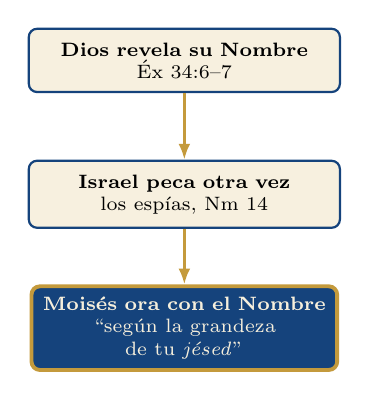
\begin{tikzpicture}[font=\scriptsize]
 \node[caja,text width=3.6cm,align=center] (a) at (0,1.7) {\textbf{Dios revela su Nombre}\\ Éx 34:6--7};
 \node[caja,text width=3.6cm,align=center] (b) at (0,0) {\textbf{Israel peca otra vez}\\ los espías, Nm 14};
 \node[draw=dorado,line width=1.4pt,fill=azul,text=papiro,rounded corners=3pt,text width=3.6cm,align=center,inner sep=4pt] (c) at (0,-1.7) {\textbf{Moisés ora con el Nombre}\\ ``según la grandeza de tu \emph{jésed}''};
 \draw[-{Latex[length=2mm]},dorado,line width=1pt](a)--(b); \draw[-{Latex[length=2mm]},dorado,line width=1pt](b)--(c);
\end{tikzpicture}
\end{column}
\end{columns}\par\medskip
\small\RaggedRight Moisés no apela a la bondad de Israel, sino al \destacar{carácter de Dios}. Aprendió en el Sinaí a orar con las palabras que Dios dijo de sí mismo. Es el patrón que tomará la oración judía (siguiente sección).
\end{frame}

% ------------------------------------------------------------------
\section{Judaísmo}

\begin{frame}{Las trece medidas de misericordia}
\centering
\begin{tikzpicture}[font=\tiny,scale=0.9]
 \node[draw=dorado,line width=1.6pt,fill=azul,text=papiro,circle,minimum size=1.5cm,align=center,font=\scriptsize\bfseries] (c) at (0,0) {\heb{שְׁלֹשׁ עֶשְׂרֵה}\\ \heb{מִדּוֹת}};
 \foreach \i/\h/\tr in {1/{יְהוָה}/{\SENOR},2/{יְהוָה}/{\SENOR},3/{אֵל}/{Dios},4/{רַחוּם}/{compasivo},5/{וְחַנּוּן}/{clemente},
   6/{אֶרֶךְ אַפַּיִם}/{lento para la ira},7/{וְרַב־חֶסֶד}/{abundante en \emph{jésed}},8/{וֶאֱמֶת}/{y verdad},
   9/{נֹצֵר חֶסֶד לָאֲלָפִים}/{guarda \emph{jésed} a millares},10/{נֹשֵׂא עָוֹן}/{carga la iniquidad},11/{וָפֶשַׁע}/{la rebelión},
   12/{וְחַטָּאָה}/{y el pecado},13/{וְנַקֵּה}/{y absuelve}}{
  \pgfmathsetmacro{\ang}{90-(\i-1)*360/13}
  \node[caja,text width=1.5cm,align=center,inner sep=1.5pt,font=\tiny] (n\i) at (\ang:4.9cm and 2.05cm) {\textbf{\textcolor{azul}{\i}}\ \heb{\h}\\ \tr};
  \draw[dorado,line width=0.6pt] (c) -- (n\i);}
\end{tikzpicture}\par\smallskip
\begin{columns}[t,onlytextwidth]
\begin{column}{0.49\textwidth}\scriptsize
El judaísmo llama a Éx 34:6--7 las \emph{shelosh esré middot}, ``trece medidas''. Cuenta de Rabbenu Tam (Tosafot a \emph{Rosh Hashaná} 17b): los dos nombres son la misericordia \emph{antes} del pecado y \emph{después} del arrepentimiento.
\end{column}
\begin{column}{0.49\textwidth}
\precision{la cuenta varía: Rabbenu Nissim no cuenta el primer nombre y divide ``guarda \emph{jésed}'' / ``a millares'' (Tosafot, ibíd.). Tu imagen comienza en \emph{El}.}
\end{column}
\end{columns}
\end{frame}

\begin{frame}{El Talmud: ``les mostró el orden de la oración''}
\begin{columns}[t,onlytextwidth]
\begin{column}{0.52\textwidth}\small
\textbf{Rabí Yojanán} (\emph{Rosh Hashaná} 17b): si el verso no estuviera escrito, sería imposible decirlo. Enseña que el Santo, bendito sea, se envolvió (en un manto de oración) como el que dirige la oración de la congregación, y le mostró a Moisés el orden de la oración. Le dijo:
\begin{center}\heb{כׇּל זְמַן שֶׁיִּשְׂרָאֵל חוֹטְאִין}\\ \heb{יַעֲשׂוּ לְפָנַי כַּסֵּדֶר הַזֶּה וַאֲנִי מוֹחֵל לָהֶם}\end{center}
``Siempre que Israel peque, que hagan delante de mí este orden, y yo los perdonaré''.
\end{column}
\begin{column}{0.46\textwidth}\small
\textbf{Rav Yehudá} (ibíd.):
\begin{center}\heb{בְּרִית כְּרוּתָה לִשְׁלֹשׁ עֶשְׂרֵה מִדּוֹת}\\ \heb{שֶׁאֵינָן חוֹזְרוֹת רֵיקָם}\end{center}
``Hay un pacto hecho con las trece medidas: no vuelven vacías'', y cita Éx 34:10: ``He aquí, yo hago pacto''.\par\medskip
\textbf{Rashi} (a Éx 34:6): ``\SENOR, \SENOR'' es la medida de misericordia, una vez antes de que el hombre peque y otra después de que peque y se arrepienta.
\end{column}
\end{columns}\par\smallskip
\precision{interpretación rabínica; texto según la edición William Davidson del Talmud en Sefaria. Es la misma lógica de Moisés en Nm 14:18--19: orar con el Nombre.}
\end{frame}

\begin{frame}{Misericordia y juicio en el Nombre}
\begin{columns}[t,onlytextwidth]
\begin{column}{0.49\textwidth}\small
\begin{itemize}
\item Los sabios distinguen dos ``medidas'': \heb{מִדַּת הָרַחֲמִים} (\emph{middat harajamim}), unida al nombre \heb{יְהוָה}, y \heb{מִדַּת הַדִּין} (\emph{middat haddín}), unida a \emph{Elohim}.
\item Rashi (a Gn 1:1): Dios pensó crear el mundo con la medida del juicio; vio que el mundo no podía subsistir, ``antepuso la medida de misericordia y la asoció a la del juicio''.
\item En el Talmud, Dios es llamado a menudo \heb{רַחֲמָנָא} (\emph{Rajmaná}), ``el Misericordioso''.
\end{itemize}
\end{column}
\begin{column}{0.49\textwidth}
\scriptsize\textbf{Targum Ónkelos} (Éx 34:6--7):
\begin{center}\heb{וּקְרָא יְיָ יְיָ אֱלָהָא רַחֲמָנָא וְחַנָּנָא}\end{center}
``y proclamó: \SENOR, \SENOR, Dios misericordioso y clemente''. Y traduce \emph{venaqqé lo yenaqqé} así:
\begin{center}\heb{סָלַח לִדְתַיְבִין לְאוֹרַיְתֵיהּ}\\ \heb{וְלִדְלָא תַיְבִין לָא מְזַכֵּי}\end{center}
``perdona a los que vuelven a su Torá, y a los que no vuelven no los absuelve''.\par\smallskip
\precision{todas son lecturas rabínicas. Ónkelos resuelve la tensión de Éx 34:7 con el arrepentimiento, igual que Pink (``Dios muestra misericordia a los verdaderamente penitentes'').}
\end{column}
\end{columns}
\end{frame}

\begin{frame}{En la oración y en el calendario}
\scriptsize\renewcommand{\arraystretch}{1.2}
\begin{tabular}{@{}>{\RaggedRight\arraybackslash}p{2.6cm}>{\RaggedRight\arraybackslash}p{9.2cm}@{}}
\toprule
\textbf{\emph{Selijot}} & oraciones penitenciales antes de Rosh Hashaná y en los ayunos: su centro es recitar las trece medidas (Elbogen, 1993). \\
\textbf{Yom Kipur} & las trece medidas se repiten a lo largo del día, hasta la oración final (\emph{Neilá}). En la tarde se lee el libro de Jonás (\emph{Meguilá} 31a): la misericordia con Nínive en el día del perdón de Israel. \\
\textbf{\emph{Ahavá rabbá}} & bendición diaria antes del \emph{Shemá}: \heb{אָבִינוּ הָאָב הָרַחֲמָן הַמְרַחֵם רַחֵם עָלֵינוּ}, ``Padre nuestro, Padre misericordioso, que tienes compasión: ten compasión de nosotros''. \\
\textbf{\emph{Tashlij}} & en Rosh Hashaná se recita Mi 7:18--20 junto a aguas: ``echará en lo profundo del mar todos nuestros pecados''. \\
\bottomrule
\end{tabular}\par\medskip
\begin{cita}¿Qué Dios como tú, que perdona la maldad, y olvida el pecado del remanente de su heredad? No retuvo para siempre su enojo, porque se deleita en misericordia.\fuente{(Mi 7:18, RVR1960)}\end{cita}
\scriptsize\heb{כִּי־חָפֵץ חֶסֶד הוּא}: ``porque se deleita en \emph{jésed}''. \heb{מִי־אֵל כָּמוֹךָ} (\emph{mi El kamoja}) es quizá un juego con el nombre del profeta, \emph{Mijá-yahu}, ``¿quién como \SENOR?''.
\end{frame}

\begin{frame}{``Sé como él'' y Qumrán}
\begin{columns}[t,onlytextwidth]
\begin{column}{0.50\textwidth}\small
\textbf{Imitar a Dios.} Abba Shaúl (\emph{Shabat} 133b), sobre ``este es mi Dios, y lo alabaré'' (Éx 15:2):
\begin{center}\heb{הֱוֵי דּוֹמֶה לוֹ}\\ \heb{מָה הוּא חַנּוּן וְרַחוּם אַף אַתָּה חַנּוּן וְרַחוּם}\end{center}
``Sé semejante a él: como él es clemente y misericordioso, sé tú también clemente y misericordioso''.\par\smallskip
\scriptsize Rabí Jamá bar Janiná (\emph{Sotá} 14a): ``andar en pos del \SENOR'' (Dt 13:4 [13:5]) es seguir sus medidas: vestir al desnudo, visitar al enfermo, consolar al que llora y sepultar al muerto, como él lo hizo.
\end{column}
\begin{column}{0.48\textwidth}\small
\textbf{Qumrán.} El rollo de los Salmos de la cueva 11 (11QSal\textsuperscript{a}) copia el Salmo 145, el acróstico que cita Éx 34:6 en el v.~8, con un estribillo después de cada verso:
\begin{center}\heb{בָּרוּךְ יְהוָה וּבָרוּךְ שְׁמוֹ לְעוֹלָם וָעֶד}\end{center}
``Bendito el \SENOR{} y bendito su nombre por siempre jamás''.\par\smallskip
\precision{según la edición de Sanders (1965, DJD IV). Conviene cotejar la imagen del rollo en la Leon Levy Dead Sea Scrolls Digital Library.}
\end{column}
\end{columns}\par\smallskip
\precision{la enseñanza de Abba Shaúl y la de Sotá 14a son el paralelo judío más cercano a ``Sed misericordiosos, como vuestro Padre'' (Lc 6:36).}
\end{frame}

% ------------------------------------------------------------------
\section{En Cristo}

\begin{frame}{Pablo cita Éxodo 33:19}
\fotolado{panel_romanos9.jpg}{Elaboración propia: Ro 9:15 en escritura uncial (texto NA28).}
\begin{columns}[c,onlytextwidth]
\begin{column}{0.58\textwidth}
\begin{cita}¿Qué, pues, diremos? ¿Que hay injusticia en Dios? En ninguna manera. Pues a Moisés dice: Tendré misericordia del que yo tenga misericordia, y me compadeceré del que yo me compadezca. Así que no depende del que quiere, ni del que corre, sino de Dios que tiene misericordia.\fuente{(Ro 9:14--16, RVR1960)}\end{cita}
\scriptsize\renewcommand{\arraystretch}{1.15}
\begin{tabular}{@{}>{\RaggedRight\arraybackslash}p{1.3cm}>{\RaggedRight\arraybackslash}p{5.4cm}@{}}
\toprule
TM & \heb{וְחַנֹּתִי אֶת־אֲשֶׁר אָחֹן וְרִחַמְתִּי אֶת־אֲשֶׁר אֲרַחֵם} \\
LXX & \grc{ἐλεήσω ὃν ἂν ἐλεῶ καὶ οἰκτιρήσω ὃν ἂν οἰκτίρω} \\
Ro 9:15 & \grc{ἐλεήσω ὃν ἂν ἐλεῶ καὶ οἰκτιρήσω ὃν ἂν οἰκτίρω} \\
\bottomrule
\end{tabular}\par\smallskip
Pablo cita la LXX palabra por palabra. Lee a Israel como Moisés: la misericordia es libre y no depende del esfuerzo humano (\grc{οὐ τοῦ θέλοντος οὐδὲ τοῦ τρέχοντος}).
\end{column}
\begin{column}{0.40\textwidth}\end{column}
\end{columns}
\end{frame}

\begin{frame}{Misericordia para todos}
\begin{columns}[t,onlytextwidth]
\begin{column}{0.49\textwidth}
\begin{cita}Porque Dios sujetó a todos en desobediencia, para tener misericordia de todos. ¡Oh profundidad de las riquezas de la sabiduría y de la ciencia de Dios!\fuente{(Ro 11:32--33, RVR1960)}\end{cita}
\scriptsize\grc{ἵνα τοὺς πάντας ἐλεήσῃ}: ``para tener misericordia de todos'', judíos y gentiles. Romanos 9--11 empieza con la cita de Éx 33:19 y termina en esta doxología.
\end{column}
\begin{column}{0.49\textwidth}
\begin{cita}y para que los gentiles glorifiquen a Dios por su misericordia, como está escrito: Por tanto, yo te confesaré entre los gentiles, Y cantaré a tu nombre.\fuente{(Ro 15:9, RVR1960)}\end{cita}
\scriptsize Cristo vino ``para mostrar la verdad de Dios'' a Israel (15:8) y para que los gentiles alaben su misericordia (15:9): \emph{emet} para Jacob, \emph{jésed} para las naciones (cf. Mi 7:20).
\end{column}
\end{columns}\par\smallskip
\centering
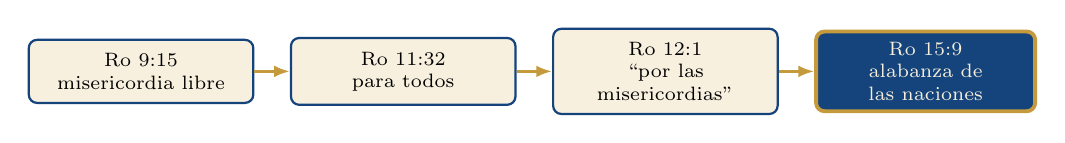
\begin{tikzpicture}[font=\scriptsize,node distance=0.45cm]
 \node[caja,text width=2.5cm,align=center] (a) {Ro 9:15\\ misericordia libre};
 \node[caja,text width=2.5cm,align=center,right=of a] (b) {Ro 11:32\\ para todos};
 \node[caja,text width=2.5cm,align=center,right=of b] (c) {Ro 12:1\\ ``por las misericordias''};
 \node[draw=dorado,line width=1.4pt,fill=azul,text=papiro,rounded corners=3pt,text width=2.5cm,align=center,inner sep=4pt,right=of c] (d) {Ro 15:9\\ alabanza de las naciones};
 \foreach \i/\j in {a/b,b/c,c/d}\draw[-{Latex[length=2mm]},dorado,line width=1pt](\i)--(\j);
\end{tikzpicture}
\end{frame}

\begin{frame}{``Padre de misericordias''}
\begin{columns}[t,onlytextwidth]
\begin{column}{0.49\textwidth}
\begin{cita}Bendito sea el Dios y Padre de nuestro Señor Jesucristo, Padre de misericordias y Dios de toda consolación.\fuente{(2~Co 1:3, RVR1960)}\end{cita}
\scriptsize\grc{ὁ πατὴρ τῶν οἰκτιρμῶν}: ``el Padre de las compasiones''. Pablo bendice a Dios con la forma de la bendición judía (\emph{barúj}) y con un título cercano a la oración de Israel: \heb{הָאָב הָרַחֲמָן}, ``el Padre misericordioso''.
\end{column}
\begin{column}{0.49\textwidth}
\begin{cita}Pero Dios, que es rico en misericordia, por su gran amor con que nos amó, aun estando nosotros muertos en pecados, nos dio vida juntamente con Cristo (por gracia sois salvos).\fuente{(Ef 2:4--5, RVR1960)}\end{cita}
\scriptsize\grc{πλούσιος ὢν ἐν ἐλέει}: ``siendo rico en misericordia'', eco del \emph{rav jésed} de Éx 34:6 (LXX \grc{πολυέλεος}).
\end{column}
\end{columns}\par\smallskip
\precision{el paralelo entre 2~Co 1:3 y la oración judía es una lectura propia; la autoría paulina de Efesios es discutida, pero el mismo título está en una carta indiscutida (2~Co 1:3).}
\end{frame}

\begin{frame}{Salvos por su misericordia}
\begin{columns}[t,onlytextwidth]
\begin{column}{0.49\textwidth}
\begin{cita}Pero cuando se manifestó la bondad de Dios nuestro Salvador, y su amor para con los hombres, nos salvó, no por obras de justicia que nosotros hubiéramos hecho, sino por su misericordia.\fuente{(Tit 3:4--5, RVR1960)}\end{cita}
\begin{cita}Pero por esto fui recibido a misericordia, para que Jesucristo mostrase en mí el primero toda su clemencia, para ejemplo de los que habrían de creer en él para vida eterna.\fuente{(1~Ti 1:16, RVR1960)}\end{cita}
\end{column}
\begin{column}{0.49\textwidth}\small
\begin{itemize}
\item \grc{κατὰ τὸ αὐτοῦ ἔλεος ἔσωσεν ἡμᾶς}: ``según su misericordia nos salvó''. Obras y misericordia se excluyen (Pink).
\item Pablo, ``blasfemo, perseguidor e injuriador'' (1~Ti 1:13), se presenta como \destacar{ejemplo}: \grc{ἠλεήθην}, ``fui objeto de misericordia''.
\item Como Moisés en el Sinaí, Pablo es un hombre que vio la gloria después de su pecado (Hch 9:3; 2~Co 4:6).
\end{itemize}
\precision{la autoría de las Pastorales es discutida; Ro 9:16 dice lo mismo en una carta indiscutida.}
\end{column}
\end{columns}
\end{frame}

\begin{frame}{La gloria que Moisés pidió}
\centering
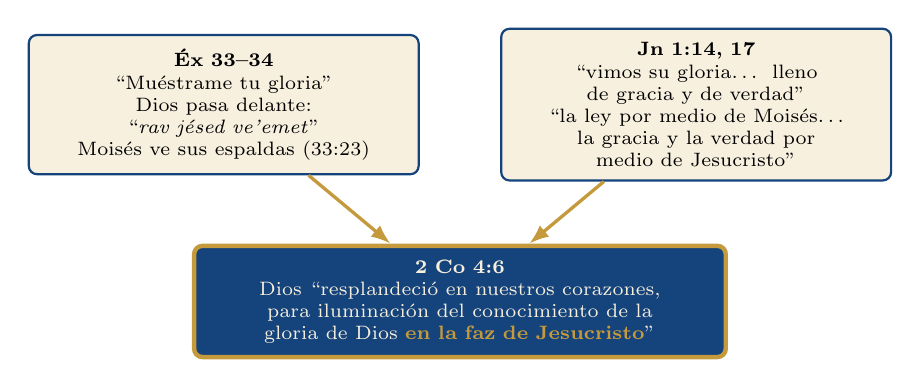
\begin{tikzpicture}[font=\scriptsize]
 \node[caja,text width=4.6cm,align=center] (m) at (-3.0,1.3) {\textbf{Éx 33--34}\\ ``Muéstrame tu gloria''\\ Dios pasa delante: ``\emph{rav jésed ve'emet}''\\ Moisés ve sus espaldas (33:23)};
 \node[caja,text width=4.6cm,align=center] (j) at (3.0,1.3) {\textbf{Jn 1:14, 17}\\ ``vimos su gloria\ldots{} lleno de gracia y de verdad''\\ ``la ley por medio de Moisés\ldots{} la gracia y la verdad por medio de Jesucristo''};
 \node[draw=dorado,line width=1.6pt,fill=azul,text=papiro,rounded corners=3pt,text width=6.4cm,align=center,inner sep=5pt] (p) at (0,-1.2) {\textbf{2 Co 4:6}\\ Dios ``resplandeció en nuestros corazones, para iluminación del conocimiento de la gloria de Dios \textbf{\textcolor{dorado}{en la faz de Jesucristo}}''};
 \draw[-{Latex[length=2.5mm]},dorado,line width=1.2pt] (m)--(p);
 \draw[-{Latex[length=2.5mm]},dorado,line width=1.2pt] (j)--(p);
\end{tikzpicture}\par\medskip
\small\RaggedRight Moisés no pudo ver el rostro (\heb{פָּנִים}, Éx 33:20). En Cristo la gloria tiene rostro, y ese rostro es misericordia. ``En él habita corporalmente toda la plenitud de la Deidad'' (Col 2:9).\par\smallskip
\precision{Pablo compara su ministerio con el de Moisés en 2~Co 3:7--4:6; la conexión con Jn 1:14 es de esta serie (Juan no es Pablo).}
\end{frame}

\begin{frame}{El propiciatorio: trono de misericordia}
\begin{columns}[t,onlytextwidth]
\begin{column}{0.49\textwidth}
\begin{cita}a quien Dios puso como propiciación por medio de la fe en su sangre, para manifestar su justicia, a causa de haber pasado por alto, en su paciencia, los pecados pasados.\fuente{(Ro 3:25, RVR1960)}\end{cita}
\scriptsize\grc{ἱλαστήριον}: en la LXX, la tapa del arca, \heb{כַּפֹּרֶת} (\emph{kapporet}), donde Dios se encontraba con Israel (Éx 25:22). Las tablas renovadas de Éx 34 se guardaron debajo de esa tapa (Dt 10:1--5).
\end{column}
\begin{column}{0.49\textwidth}
\begin{cita}Acerquémonos, pues, confiadamente al trono de la gracia, para alcanzar misericordia y hallar gracia para el oportuno socorro.\fuente{(He 4:16, RVR1960)}\end{cita}
\small En la cruz, ``la misericordia y la verdad se encontraron'' (Sal 85:10): Dios perdona sin dejar de ser justo, ``el justo, y el que justifica'' (Ro 3:26).\par\smallskip
\precision{la autoría de Hebreos es desconocida; no es de Pablo. La ley bajo la tapa de misericordia es una imagen tipológica propia.}
\end{column}
\end{columns}
\end{frame}

% ------------------------------------------------------------------
\section{Vivirlo}

\begin{frame}{Un atributo comunicable}
\begin{columns}[t,onlytextwidth]
\begin{column}{0.49\textwidth}
\begin{cita}Sed, pues, misericordiosos, como también vuestro Padre es misericordioso.\fuente{(Lc 6:36, RVR1960)}\end{cita}
\scriptsize\grc{γίνεσθε οἰκτίρμονες καθὼς ὁ πατὴρ ὑμῶν οἰκτίρμων ἐστίν}. \grc{οἰκτίρμων} es la palabra de la LXX para \emph{rajum} en Éx 34:6: Jesús pide a sus discípulos el primer rasgo del Nombre.
\begin{cita}Bienaventurados los misericordiosos, porque ellos alcanzarán misericordia.\fuente{(Mt 5:7, RVR1960)}\end{cita}
\end{column}
\begin{column}{0.49\textwidth}\small
\begin{itemize}
\item La misericordia es \destacar{comunicable}: el ser humano puede reflejarla, no producirla.
\item Se recibe primero y se da después: ``alcanzarán misericordia'' (\grc{ἐλεηθήσονται}, pasivo: Dios la da).
\item Abba Shaúl lo dijo en Israel: ``como él es clemente y misericordioso, sé tú también''.
\end{itemize}
\begin{cita}Oh hombre, él te ha declarado lo que es bueno, y qué pide \SENOR{} de ti: solamente hacer justicia, y amar misericordia, y humillarte ante tu Dios.\fuente{(Mi 6:8, RVR1960)}\end{cita}
\end{column}
\end{columns}
\end{frame}

\begin{frame}{¿Quién no alcanzará misericordia?}
\begin{columns}[t,onlytextwidth]
\begin{column}{0.49\textwidth}
\begin{cita}Porque juicio sin misericordia se hará con aquel que no hiciere misericordia; y la misericordia triunfa sobre el juicio.\fuente{(Stg 2:13, RVR1960)}\end{cita}
\scriptsize\grc{ἡ γὰρ κρίσις ἀνέλεος τῷ μὴ ποιήσαντι ἔλεος· κατακαυχᾶται ἔλεος κρίσεως}. \grc{ἀνέλεος}: ``sin misericordia''; \grc{κατακαυχᾶται}: ``se gloría por encima de, triunfa''.\par\medskip
\small Aquí se afirma claramente que el que no muestra misericordia será juzgado sin ella.
\end{column}
\begin{column}{0.49\textwidth}
\begin{cita}¿No debías tú también tener misericordia de tu consiervo, como yo tuve misericordia de ti? Entonces su señor, enojado, le entregó a los verdugos\ldots{}\fuente{(Mt 18:33--34, RVR1960)}\end{cita}
\scriptsize Diez mil talentos perdonados, cien denarios exigidos (Mt 18:24, 28). El siervo recibió \emph{janán} y no lo dio. Santiago, judío, dice lo mismo que Éx 34:7: la misericordia es abundante, pero no se burla de ella.\par\smallskip
\precision{Santiago no es de Pablo; está en tu material.}
\end{column}
\end{columns}
\end{frame}

\begin{frame}{``Ve, y haz tú lo mismo''}
\begin{columns}[t,onlytextwidth]
\begin{column}{0.52\textwidth}
\begin{cita}Pero un samaritano, que iba de camino, vino cerca de él, y viéndole, fue movido a misericordia; y acercándose, vendó sus heridas, echándoles aceite y vino\ldots{} ¿Quién, pues, de estos tres te parece que fue el prójimo del que cayó en manos de los ladrones? El dijo: El que usó de misericordia con él. Entonces Jesús le dijo: Ve, y haz tú lo mismo.\fuente{(Lc 10:33--37, RVR1960)}\end{cita}
\end{column}
\begin{column}{0.46\textwidth}\scriptsize
\renewcommand{\arraystretch}{1.15}
\begin{tabular}{@{}>{\RaggedRight\arraybackslash}p{2.0cm}>{\RaggedRight\arraybackslash}p{3.3cm}@{}}
\toprule
\grc{ἐσπλαγχνίσθη} (10:33) & se conmovió en las entrañas: \emph{rajamím} \\
\grc{ὁ ποιήσας τὸ ἔλεος} (10:37) & ``el que hizo misericordia'': el hebreo \heb{עָשָׂה חֶסֶד} (\emph{asá jésed}) \\
\bottomrule
\end{tabular}\par\medskip
\small Un escriba pregunta ``¿quién es mi prójimo?'' (10:29). Jesús da vuelta la pregunta: no es a quién debo amar, sino \destacar{de quién me hago prójimo}. La misericordia se siente (entrañas) y se hace (\emph{asá jésed}).
\end{column}
\end{columns}
\end{frame}

\begin{frame}{Siquem: el pacto sin \emph{jésed}}
\begin{columns}[t,onlytextwidth]
\begin{column}{0.52\textwidth}
\begin{cita}Pero aconteció que cuando murió Gedeón, los hijos de Israel volvieron a prostituirse yendo tras los baales, y escogieron por dios a Baal-berit. Y no se acordaron los hijos de Israel de \SENOR{} su Dios, que los había librado de todos sus enemigos en derredor; ni se mostraron agradecidos con la casa de Jerobaal, el cual es Gedeón, conforme a todo el bien que él había hecho a Israel.\fuente{(Jue 8:33--35, RVR1960)}\end{cita}
\end{column}
\begin{column}{0.46\textwidth}\scriptsize
\renewcommand{\arraystretch}{1.15}
\begin{tabular}{@{}>{\RaggedRight\arraybackslash}p{2.1cm}>{\RaggedRight\arraybackslash}p{3.2cm}@{}}
\toprule
\heb{בַּעַל בְּרִית} \emph{Ba'al berit} & ``señor del pacto'': un dios cananeo del pacto, en Siquem \\
\heb{אֵל בְּרִית} \emph{El berit} & ``dios del pacto''; su templo (9:4, 46) \\
\heb{וְלֹא־עָשׂוּ חֶסֶד} & ``y no hicieron \emph{jésed}'' (RVR1960: ``ni se mostraron agradecidos'') \\
\bottomrule
\end{tabular}\par\medskip
\small En Siquem, Abram había dicho ``no'' a los dioses de la tierra (Gn 12:6--7). Siglos después, Israel cambió al Dios del pacto por un ``señor del pacto''. Quien olvida el \emph{jésed} de Dios deja de hacer \emph{jésed} a los demás.
\end{column}
\end{columns}
\precision{el vínculo entre 8:34 y 8:35 está en el texto; leer Baal-berit como imitación del pacto es interpretación (Block, 1999).}
\end{frame}

\begin{frame}{Cuatro respuestas a la misericordia}
\centering
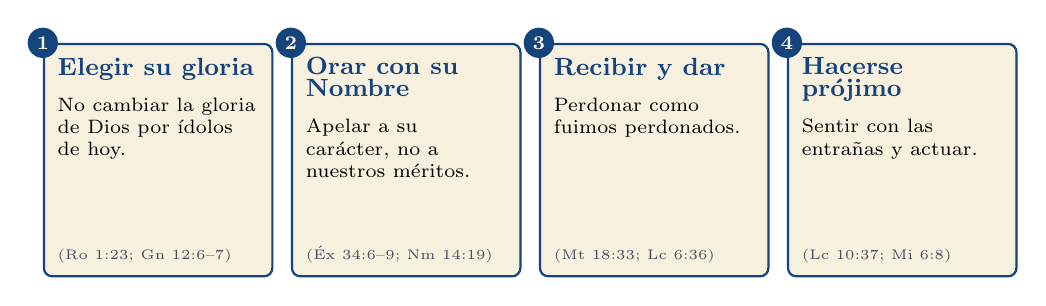
\begin{tikzpicture}
 \foreach \x/\n/\t/\d/\r in {0/1/{Elegir su gloria}/{No cambiar la gloria de Dios por ídolos de hoy.}/{Ro 1:23; Gn 12:6--7},
   3.15/2/{Orar con su Nombre}/{Apelar a su carácter, no a nuestros méritos.}/{Éx 34:6--9; Nm 14:19},
   6.3/3/{Recibir y dar}/{Perdonar como fuimos perdonados.}/{Mt 18:33; Lc 6:36},
   9.45/4/{Hacerse prójimo}/{Sentir con las entrañas y actuar.}/{Lc 10:37; Mi 6:8}}{
  \node[caja,anchor=north] (b\n) at (\x,0) {\parbox[t][2.6cm][t]{2.55cm}{\RaggedRight
    {\small\textbf{\textcolor{azul}{\t}}}\\[5pt]\scriptsize \d\par\vfill{\tiny\color{gris}(\r)}}};
  \node[circle,fill=azul,text=papiro,font=\scriptsize\bfseries,inner sep=1.6pt] at (b\n.north west) {\n};}
\end{tikzpicture}\par\medskip
\begin{cita}Así que, hermanos, os ruego por las misericordias de Dios, que presentéis vuestros cuerpos en sacrificio vivo, santo, agradable a Dios, que es vuestro culto racional.\fuente{(Ro 12:1, RVR1960)}\end{cita}
\scriptsize\grc{διὰ τῶν οἰκτιρμῶν τοῦ θεοῦ}: toda la ética de Romanos 12--15 se apoya en las misericordias expuestas en Romanos 1--11.
\end{frame}

% ------------------------------------------------------------------
\section{Síntesis}

\begin{frame}{Síntesis}
\begin{tcolorbox}[colback=papiro,colframe=azul,boxrule=1pt,arc=3pt]
\small Cuando Israel cambió su gloria por un becerro, Dios mostró la suya: ``¡\SENOR! ¡\SENOR! fuerte, misericordioso y piadoso'' (Éx 34:6). Su misericordia es \destacar{gracia} libre (\emph{janán}), \destacar{amor leal} (\emph{jésed}), \destacar{ternura} de entrañas (\emph{rajamím}) y \destacar{clemencia} que saca del juicio (\emph{jamal}), sin dejar de ser justa. Israel la convirtió en su oración; Pablo la vio en el rostro de Cristo (2~Co 4:6), ``Padre de misericordias'' (2~Co 1:3). Quien la recibe, la refleja (Lc 6:36).
\end{tcolorbox}
\scriptsize\renewcommand{\arraystretch}{1.15}
\begin{tabular}{@{}>{\RaggedRight\arraybackslash}p{2.4cm}>{\RaggedRight\arraybackslash}p{9.4cm}@{}}
\toprule
\textbf{Mirada} & \textbf{Aporte} \\ \midrule
Hebrea & cuatro palabras; el Nombre de Éx 34:6--7; Moisés intercede con el Nombre; Lot, Efraín, Nínive. \\
Judía & las trece medidas; ``les mostró el orden de la oración''; \emph{Rajmaná}; ``sé como él'' (Abba Shaúl). \\
Pink & nace de la bondad; presupone la miseria; general, especial y soberana; no se presume. \\
Paulina & Ro 9:15 = Éx 33:19; misericordia para todos (Ro 11:32); Padre de misericordias; salvos por su misericordia. \\
\bottomrule
\end{tabular}
\end{frame}

\begin{frame}{Para la reflexión}
\begin{cita}Mas alábese en esto el que se hubiere de alabar: en entenderme y conocerme, que yo soy \SENOR, que hago misericordia, juicio y justicia en la tierra; porque estas cosas quiero, dice \SENOR.\fuente{(Jer 9:24 [9:23], RVR1960)}\end{cita}
\begin{center}\heb{כִּי אֲנִי יְהוָה עֹשֶׂה חֶסֶד מִשְׁפָּט וּצְדָקָה בָּאָרֶץ}\end{center}
\small
\begin{itemize}
\item ¿Qué ``gloria'' he puesto en lugar de la gloria de Dios?
\item Cuando oro después de pecar, ¿apelo a mis promesas o a su Nombre?
\item ¿A quién le estoy cobrando cien denarios después de que me perdonaron diez mil talentos?
\item ¿De quién me estoy haciendo prójimo esta semana?
\end{itemize}
\end{frame}

% ------------------------------------------------------------------
\section{Glosario}

\begin{frame}{Glosario (1)}
\scriptsize
\begin{columns}[t,onlytextwidth]
\begin{column}{0.49\textwidth}
\begin{description}\setlength{\itemsep}{1pt}
\item[\emph{Anéleos}] (\grc{ἀνέλεος}) sin misericordia (Stg 2:13).
\item[\emph{Éleos}] (\grc{ἔλεος}) misericordia, compasión activa; en la LXX traduce \emph{jésed}.
\item[\emph{Eleēmōn}] (\grc{ἐλεήμων}) misericordioso (Mt 5:7; He 2:17).
\item[\emph{Emet}] (\heb{אֱמֶת}) verdad, firmeza, fidelidad.
\item[\emph{Eúsplanjnos}] (\grc{εὔσπλαγχνος}) ``de buenas entrañas'' (Ef 4:32).
\item[\emph{Hósios}] (\grc{ὅσιος}) leal, santo; \emph{ta hósia}, las lealtades (Hch 13:34).
\item[\emph{Janán}] (\heb{חָנַן}) inclinarse con favor; tener gracia.
\item[\emph{Jamal}] (\heb{חָמַל}) compadecerse; perdonar la vida.
\item[\emph{Jasid}] (\heb{חָסִיד}) misericordioso, el hombre de \emph{jésed}.
\item[\emph{Jésed}] (\heb{חֶסֶד}) amor leal del pacto.
\item[\emph{Jus}] (\heb{חוּס}) tener lástima, perdonar (Jon 4:11).
\end{description}
\end{column}
\begin{column}{0.49\textwidth}
\begin{description}\setlength{\itemsep}{1pt}
\item[\emph{Kavod}] (\heb{כָּבוֹד}) gloria; ``peso''.
\item[\emph{Middat harajamim}] (\heb{מִדַּת הָרַחֲמִים}) la medida de misericordia.
\item[\emph{Nijam}] (\heb{נִחַם}) conmoverse, cambiar el curso (Jue 2:18).
\item[\emph{Oiktirmós}] (\grc{οἰκτιρμός}) compasión (2~Co 1:3; Ro 12:1).
\item[\emph{Polýsplanjnos}] (\grc{πολύσπλαγχνος}) ``de muchas entrañas'' (Stg 5:11).
\item[\emph{Rajamím}] (\heb{רַחֲמִים}) entrañas; compasión.
\item[\emph{Rajmaná}] (\heb{רַחֲמָנָא}) ``el Misericordioso'', nombre de Dios en el Talmud.
\item[\emph{Rajum}] (\heb{רַחוּם}) compasivo (Éx 34:6).
\item[\emph{Réjem}] (\heb{רֶחֶם}) vientre, matriz.
\item[\emph{Selijot}] (\heb{סְלִיחוֹת}) oraciones penitenciales judías.
\item[\emph{Shelosh esré middot}] (\heb{שְׁלֹשׁ עֶשְׂרֵה מִדּוֹת}) las trece medidas.
\end{description}
\end{column}
\end{columns}
\end{frame}

\begin{frame}{Glosario (2)}
\scriptsize
\begin{description}\setlength{\itemsep}{1pt}
\item[\emph{Splánjna}] (\grc{σπλάγχνα}) entrañas; ``entrañable misericordia'' (Lc 1:78; Col 3:12).
\item[\emph{Splanjnízomai}] (\grc{σπλαγχνίζομαι}) conmoverse en las entrañas.
\item[\emph{Tejinná}, \emph{tajanunim}] (\heb{תְּחִנָּה}, \heb{תַּחֲנוּנִים}) súplica; la gracia que se pide (Esd 9:8; Jer 31:9).
\item[\emph{Tov ayin}] (\heb{טוֹב־עַיִן}) ``bueno de ojo'': generoso, misericordioso (Pr 22:9).
\end{description}
\end{frame}

% ------------------------------------------------------------------
\section{Referencias}

\begin{frame}{Referencias}
\fontsize{5.6}{6.6}\selectfont
\refapa{Bauer, W., Danker, F.~W., Arndt, W.~F., \& Gingrich, F.~W. (2000). \emph{A Greek-English lexicon of the New Testament and other early Christian literature} (3.ª ed.). University of Chicago Press. [BDAG]}
\refapa{\emph{Biblia Reina-Valera 1960}. (1960). Sociedades Bíblicas en América Latina.}
\refapa{Block, D.~I. (1999). \emph{Judges, Ruth}. Broadman \& Holman.}
\refapa{Carson, D.~A. (1991). \emph{The Gospel according to John}. Eerdmans.}
\refapa{Elbogen, I. (1993). \emph{Jewish liturgy: A comprehensive history} (R.~P. Scheindlin, Trad.). Jewish Publication Society.}
\refapa{Elliger, K., \& Rudolph, W. (Eds.). (1997). \emph{Biblia Hebraica Stuttgartensia} (5.ª ed.). Deutsche Bibelgesellschaft.}
\refapa{Koehler, L., \& Baumgartner, W. (2001). \emph{The Hebrew and Aramaic lexicon of the Old Testament} (M.~E.~J. Richardson, Trad.; Ed. de estudio). Brill. [HALOT]}
\refapa{Moo, D.~J. (1996). \emph{The epistle to the Romans}. Eerdmans.}
\refapa{Nestle, E., \& Aland, K. (2012). \emph{Novum Testamentum Graece} (28.ª ed.). Deutsche Bibelgesellschaft.}
\refapa{Pink, A.~W. (2020). \emph{Los atributos de Dios}. Chapel Library. (Obra original publicada en 1930)}
\refapa{Rahlfs, A., \& Hanhart, R. (Eds.). (2006). \emph{Septuaginta} (Ed. rev.). Deutsche Bibelgesellschaft.}
\refapa{Rashi. (s.f.). \emph{Comentario a Génesis y Éxodo}. Sefaria. https://www.sefaria.org}
\refapa{Sanders, J.~A. (1965). \emph{The Psalms scroll of Qumrân Cave 11 (11QPs\textsuperscript{a})} (Discoveries in the Judaean Desert IV). Clarendon Press.}
\refapa{Steinsaltz, A. (Ed.). (2017). \emph{Koren Talmud Bavli: Edición William Davidson} [Rosh Hashaná 17b; Shabat 133b; Sotá 14a; Meguilá 31a]. Sefaria. https://www.sefaria.org}
\refapa{Strong, J. (1890). \emph{The exhaustive concordance of the Bible}. Hunt \& Eaton.}
\refapa{\emph{Targum Ónkelos} [Éxodo 34]. (s.f.). Sefaria. https://www.sefaria.org}
\refapa{Wenham, G.~J. (1987). \emph{Genesis 1--15}. Word.}
\par\smallskip{\color{gris}Las citas bíblicas son de la Reina-Valera 1960; ``Jehová'' se reemplaza por \SENOR. Hebreo: BHS; griego: NA28 y LXX de Rahlfs-Hanhart. Fuentes judías: Sefaria; lo rabínico se marca como \emph{precisión}.}
\end{frame}

\end{document}
